%% LyX 2.0.6 created this file.  For more info, see http://www.lyx.org/.
%% Do not edit unless you really know what you are doing.
\documentclass[french]{amsbook}
\usepackage[T1]{fontenc}
\usepackage[utf-8]{inputenc}
\setlength{\parskip}{\smallskipamount}
\setlength{\parindent}{0pt}
\usepackage{textcomp}
\usepackage{url}
\usepackage{amsthm}
\usepackage{amstext}
\usepackage{amssymb}
\usepackage{graphicx}

\makeatletter

%%%%%%%%%%%%%%%%%%%%%%%%%%%%%% LyX specific LaTeX commands.
%% Because html converters don't know tabularnewline
\providecommand{\tabularnewline}{\\}

%%%%%%%%%%%%%%%%%%%%%%%%%%%%%% Textclass specific LaTeX commands.
\numberwithin{section}{chapter}
\numberwithin{equation}{section}
\numberwithin{figure}{section}
\theoremstyle{plain}
\newtheorem{thm}{\protect\theoremname}
  \theoremstyle{definition}
  \newtheorem{problem}[thm]{\protect\problemname}
  \theoremstyle{definition}
  \newtheorem*{problem*}{\protect\problemname}
\newenvironment{lyxcode}
{\par\begin{list}{}{
\setlength{\rightmargin}{\leftmargin}
\setlength{\listparindent}{0pt}% needed for AMS classes
\raggedright
\setlength{\itemsep}{0pt}
\setlength{\parsep}{0pt}
\normalfont\ttfamily}%
 \item[]}
{\end{list}}
 \theoremstyle{definition}
 \newtheorem*{defn*}{\protect\definitionname}
  \theoremstyle{definition}
  \newtheorem{xca}[thm]{\protect\exercisename}
  \theoremstyle{definition}
  \newtheorem*{example*}{\protect\examplename}
  \theoremstyle{definition}
  \newtheorem{example}[thm]{\protect\examplename}
  \theoremstyle{remark}
  \newtheorem{rem}[thm]{\protect\remarkname}
  \theoremstyle{definition}
  \newtheorem{defn}[thm]{\protect\definitionname}
  \theoremstyle{plain}
  \newtheorem*{prop*}{\protect\propositionname}
  \theoremstyle{remark}
  \newtheorem*{rem*}{\protect\remarkname}
  \theoremstyle{plain}
  \newtheorem*{thm*}{\protect\theoremname}
  \theoremstyle{definition}
  \newtheorem*{xca*}{\protect\exercisename}
  \theoremstyle{plain}
  \newtheorem*{lem*}{\protect\lemmaname}
  \theoremstyle{plain}
  \newtheorem{prop}[thm]{\protect\propositionname}
  \theoremstyle{plain}
  \newtheorem{algorithm}[thm]{\protect\algorithmname}

%%%%%%%%%%%%%%%%%%%%%%%%%%%%%% User specified LaTeX commands.
\usepackage{a4wide}
\newcommand{\N}{\mathbb{N}}
\newcommand{\Z}{\mathbb{Z}}
\newcommand{\Q}{\mathbb{Q}}
\newcommand{\R}{\mathbb{R}}
\newcommand{\C}{\mathbb{C}}
\usepackage{hyperref}
\makeatletter
% Yucky bugware to make hyperref and babel[francais] work together
\def\url#1{{\selectlanguage{american}\hyper@normalise\url@{#1}}}
\def\href#1#2{{\selectlanguage{american}\hyper@normalise\href@{#1}{#2}}}
\makeatother
\newcommand{\solution}{ \hrule\vspace{4cm}\hrule}

\makeatother

\usepackage{babel}
\makeatletter
\addto\extrasfrench{%
   \providecommand{\og}{\leavevmode\flqq~}%
   \providecommand{\fg}{\ifdim\lastskip>\z@\unskip\fi~\frqq}%
}

\makeatother
  \providecommand{\algorithmname}{Algorithme}
  \providecommand{\definitionname}{Définition}
  \providecommand{\examplename}{Exemple}
  \providecommand{\exercisename}{Exercice}
  \providecommand{\lemmaname}{Lemme}
  \providecommand{\problemname}{Problème}
  \providecommand{\propositionname}{Proposition}
  \providecommand{\remarkname}{Remarque}
  \providecommand{\theoremname}{Théorème}
\providecommand{\theoremname}{Théorème}

\begin{document}

\chapter{Programmation linéaire}


\section{Qu'est-ce que la programmation linéaire}


\subsection{Exemple: le problème du régime de Polly \cite[p.3]{Chvatal_LP}}
\begin{itemize}
\item Besoins journaliers:

\begin{description}
\item [{Énergie}] 2000 kcal
\item [{Protéines}] 55g
\item [{Calcium}] 800 mg
\end{description}
\item Nourriture disponible


\begin{tabular}{|c|c|c|c|c|c|}
\hline 
 & Portion & Énergie (kcal) & Protéines (g) & Calcium (mg) & Prix/portion\tabularnewline
\hline 
\hline 
Céréales & 28g & 110 & 4 & 2 & 3\tabularnewline
\hline 
Poulet & 100g & 205 & 32 & 12 & 24\tabularnewline
\hline 
Oeufs & 2 gros & 160 & 13 & 54 & 13\tabularnewline
\hline 
Lait entier & 237cc & 160 & 8 & 285 & 9\tabularnewline
\hline 
Tarte & 170g & 420 & 4 & 22 & 20\tabularnewline
\hline 
Porc et haricots & 260g & 260 & 14 & 80 & 19\tabularnewline
\hline 
\end{tabular}

\end{itemize}
Quels choix pour Polly ?
\begin{itemize}
\item Contraintes:

\begin{description}
\item [{Céréales}] au plus 4 portions par jour
\item [{Poulet}] au plus 3 portions par jour
\item [{Oeufs}] au plus 2 portions par jour
\item [{Lait}] au plus 8 portions par jour
\item [{Tarte}] au plus 2 portions par jour
\item [{Porc~et~haricots}] au plus 2 portions par jour
\end{description}
\end{itemize}
\begin{problem}
Polly peut-elle trouver une solution ?

Comment formaliser le problème ? (modélisation)

Qu'est-ce qui fait la spécificité du problème ?

Savez-vous résoudre des problèmes similaires ?
\end{problem}
%

%

%

%

%

%

%

\solution


\subsection{Forme standard d'un problème de programmation linéaire}
\begin{problem*}
\cite[p. 5]{Chvatal_LP}
\begin{lyxcode}
Maximiser:~~~~~~~~~~~~5{*}x1~+~4{*}x2~+~3{*}x3

Sous~les~contraintes:~2{*}x1~+~3{*}x2~+~~~x3~<=~~5~

~~~~~~~~~~~~~~~~~~~~~~4{*}x1~+~~~x2~+~2{*}x3~<=~11

~~~~~~~~~~~~~~~~~~~~~~3{*}x1~+~4{*}x2~+~2{*}x3~<=~~8

~~~~~~~~~~~~~~~~~~~~~~x1,~x2,~x3~>=~0



Minimiser:~~~~~~~~~~~~3{*}x1~-~~~x2

Sous~les~contraintes:~-~x1~+~6{*}x2~-~~~x3~+~~~x4~>=~-3~

~~~~~~~~~~~~~~~~~~~~~~~~~~~~~7{*}x2~~~~~~~~+~2{*}x4~=~~~5

~~~~~~~~~~~~~~~~~~~~~~~~x1~+~~~x2~+~~~x3~~~~~~~~=~~~1

~~~~~~~~~~~~~~~~~~~~~~~~~~~~~~~~~~~~~~x3~+~~~x4~<=~~2

~~~~~~~~~~~~~~~~~~~~~~~x2,~x3~>=~0
\end{lyxcode}
\end{problem*}
\begin{defn*}
Problème de programmation linéaire sous \emph{forme standard:}

Maximiser:

\[
z:=\sum_{j=1}^{n}c_{j}x_{j}
\]


Sous les contraintes:

\[
\sum_{j=1}^{n}a_{ij}x_{j}\leq b_{i},\textrm{ pour }i=1,\ldots,m
\]
 

\[
x_{j}\geq0,\textrm{ pour }j=1,\ldots,n
\]


Un choix des variables $(x_{1},\ldots,x_{n})$ est appelé \emph{solution}
du problème.

Une solution est \emph{faisable} si elle vérifie les contraintes.

$z$ est appelé \emph{fonction objective}. À chaque solution elle
associe une valeur.

Une solution est \emph{optimale} si elle est faisable et maximize
la fonction objective.\end{defn*}
\begin{xca}
Peut-on mettre sous forme standard les exemples précédents ?
\end{xca}

\subsection{Existence de solutions optimales ?}
\begin{problem}
\cite[p. 7]{Chvatal_LP}

On considère les quatre problèmes de programmation linéaire standard
suivants, écrits avec la syntaxe du système de calcul formel \texttt{MuPAD}:
\begin{lyxcode}
Chvatal7a~:=~{[}~{[}~~~x1~~~~~~<=~3,~

~~~~~~~~~~~~~~~~~~~~~~~~x2~<=~7~{]},

~~~~~~~~~~~~~~~~3~+x1~~+x2,~

~~~~~~~~~~~~~~~Nonnegative{]}:~

Chvatal7b~:=~{[}~{[}~~~x1~~+x2~<=~2,~

~~~~~~~~~~~~~~~~-2{*}x1-2{*}x2~<=~-10~{]},

~~~~~~~~~~~~~~~~~3{*}x1~~-x2,~

~~~~~~~~~~~~~~~NonNegative{]}:~

Chvatal7c~:=~{[}~{[}-2{*}x1~~+x2~<=~-1,~

~~~~~~~~~~~~~~~~~~-x1-2{*}x2~<=~-2~{]},

~~~~~~~~~~~~~~~~~~~x1~~-x2,

~~~~~~~~~~~~~~~NonNegative{]}:

extra~~~~~:=~{[}~{[}~~~x1~~+x2~<=~1~{]},

~~~~~~~~~~~~~~~~~~~x1~~+x2,

~~~~~~~~~~~~~~~NonNegative{]}:
\end{lyxcode}
\end{problem}
\begin{lyxcode}
\end{lyxcode}
\begin{problem}
Déterminer pour ces trois problèmes s'il y a des solutions optimales.\end{problem}
\begin{lyxcode}
%

%

%

%

%

%

\solution\end{lyxcode}
\begin{itemize}
\item Premier cas: une solution optimale unique
\item Deuxième cas: pas de solution faisable
\item Troisième cas: pas de solution optimale, car on peut faire tendre
la fonction objective vers l'infini avec des solutions faisables.
\item Quatrième cas: une infinité de solutions optimales.
\end{itemize}

\section{Algorithme du simplexe}


\subsection{Une pointe d'algèbre linéaire}
\begin{problem}
Considérons le système suivant:
\begin{lyxcode}
5~~=~s1~~~~~~~+~2{*}x1~+~3{*}x2~+~~~x3

11~=~~~~s2~~~~+~4{*}x1~+~~~x2~+~2{*}x3

8~~=~~~~~~~s3~+~3{*}x1~+~4{*}x2~+~2{*}x3
\end{lyxcode}
Que peut-on dire dessus?















C'est un système \emph{linéaire} à 6 inconnues et 3 équations.

L'ensemble des solutions est un sous espace de dimension $3$ de $\mathbb{R}^{3}$,
que l'on peut décrire en prenant comme paramètres \texttt{x1}, \texttt{x2}
et \texttt{x3}.

En effet, vu la forme triangulaire, \texttt{s1}, \texttt{s2} et \texttt{s3}
s'expriment en fonction de \texttt{x1}, \texttt{x2} et \texttt{x3}.

Transformer le système pour prendre comme paramètres $ $\texttt{s1},
\texttt{s2}, et \texttt{x1}.
\end{problem}

\subsection{Premier problème}
\begin{problem}
\label{probleme:simplexe1}\cite[p. 13]{Chvatal_LP}
\begin{lyxcode}
Chvatal13~:=~{[}\{2{*}x1~+~3{*}x2~+~~~x3~<=~5,~

~~~~~~~~~~~~~~~4{*}x1~+~~~x2~+~2{*}x3~<=~11,~

~~~~~~~~~~~~~~~3{*}x1~+~4{*}x2~+~2{*}x3~<=~8~~\},~

~~~~~~~~~~~~~~~5{*}x1~+~4{*}x2~+~3{*}x3,~

~~~~~~~~~~~~~~NonNegative{]}:
\end{lyxcode}
\end{problem}
Solution faisable ?

Amélioration de la solution ?

%

%

%

%

%

%

\solution

Introduction de variables d'écart:
\begin{lyxcode}
5~~=~s1~~~~~~~+~2{*}x1~+~3{*}x2~+~~~x3

11~=~~~~s2~~~~+~4{*}x1~+~~~x2~+~2{*}x3

8~~=~~~~~~~s3~+~3{*}x1~+~4{*}x2~+~2{*}x3

-{}-{}-{}-{}-{}-{}-{}-{}-{}-{}-{}-{}-{}-{}-{}-{}-{}-{}-{}-{}-{}-{}-{}-{}-{}-{}-{}-{}-{}-{}-{}-{}-{}-

z~~=~~~~~~~~~~~~5{*}x1~+~4{*}x2~+~3{*}x3
\end{lyxcode}
En augmentant x1 jusqu'à $5/2$, on fait tomber s1 à zéro.

On transforme le système, pour se ramener à une situation similaire
à la précédente:
\begin{lyxcode}
5/2~=~x1~~~~~~~+~3/2{*}x2~+~1/2{*}x3~+~1/2{*}s1

1~~~=~~~~s2~~~~-~~~5{*}x2~~~~~~~~~~~~-~2{*}s1

1/2~=~~~~~~~s3~-~1/2{*}x2~+~1/2{*}x3~-~3/2{*}s1

-{}-{}-{}-{}-{}-{}-{}-{}-{}-{}-{}-{}-{}-{}-{}-{}-{}-{}-{}-{}-{}-{}-{}-{}-{}-{}-{}-{}-{}-{}-{}-{}-{}-{}-{}-{}-{}-{}-{}-{}-

z~~~=~25/2~~~~~-~7/2~x2~+~1/2{*}x3~-~5/2{*}s1
\end{lyxcode}
On augmente x3 jusqu'à 1, ce qui fait tomber s3 à 0:
\begin{lyxcode}
1~=~x3~~~~~~~-~~~x2~-~3{*}s1~+~2{*}s3

2~=~~~~x1~~~~+~2{*}x2~+~2{*}s1~-~~~s3

1~=~~~~~~~s2~-~5{*}x2~-~2{*}s1

-{}-{}-{}-{}-{}-{}-{}-{}-{}-{}-{}-{}-{}-{}-{}-{}-{}-{}-{}-{}-{}-{}-{}-{}-{}-{}-{}-{}-{}-{}-{}-{}-

z~=~13~~~~~~~-~3{*}x2~-~~~s1~-~~~s3
\end{lyxcode}
Et maintenant, que fait-on ?


\subsection{Variables d'écart}
\begin{problem}
Est-ce que l'introduction de ces variables change le problème ?
\end{problem}

\subsection{Tableaux}
\begin{problem}
\cite[p. 19]{Chvatal_LP}
\begin{lyxcode}
Chvatal19~:=~{[}{[}~~x1~+~3{*}x2~~~+~x3~<=~3,~

~~~~~~~~~~~~~~~~-x1~~~~~~~~~+3{*}x3~<=~2,

~~~~~~~~~~~~~~~2{*}x1~+~3{*}x2~~~-~x3~<=~2,~

~~~~~~~~~~~~~~~2{*}x1~~~-~x2~+~2{*}x3~<=~4{]},~

~~~~~~~~~~~~~~~5{*}x1~+~5{*}x2~+~3{*}x3,~

~~~~~~~~~~~~~~NonNegative{]}:
\end{lyxcode}
\end{problem}
\begin{defn*}
\emph{Tableau initial:}

\[
b_{i}=s_{i}+\sum_{j=1}^{n}a_{ij}x_{j},\textrm{ pour }i=1,\ldots,m
\]


\[
z=\sum_{j=1}^{n}c_{j}x_{j}
\]


Ou sous forme matricielle:
\begin{eqnarray*}
B & =S+ & AX\\
z & = & CX\\
X & \geq & 0
\end{eqnarray*}
\end{defn*}
\begin{example*}
Tableau initial du problème précédent:
\begin{lyxcode}
3~=~s1~~~~~~~~~+~x1~+~3~x2~~~+~x3

2~=~~~s2~~~~~~~-~x1~~~~~~~~+~3~x3

2~=~~~~~s3~~~+~2~x1~+~3~x2~~~-~x3

4~=~~~~~~~s4~+~2~x1~~~-~x2~+~2~x3

-{}-{}-{}-{}-{}-{}-{}-{}-{}-{}-{}-{}-{}-{}-{}-{}-{}-{}-{}-{}-{}-{}-{}-{}-{}-{}-{}-{}-{}-{}-{}-{}-

z~=~0~~~~~~~~+~5~x1~+~5~x2~+~3~x3
\end{lyxcode}
\end{example*}
\begin{example}
On peut l'abréger sous forme matricielle: 
\begin{lyxcode}
read(\textquotedbl{}tableaux.mu\textquotedbl{}):

linopt::Transparent(Chvatal19);

+-~~~~~~~~~~~~~~~~~~~~~~~~~~~~~~~~~~~~~~~~~~~~~~~~~~~-+

|\textquotedbl{}linopt\textquotedbl{},\textquotedbl{}restr\textquotedbl{},slk{[}1{]},slk{[}2{]},slk{[}3{]},slk{[}4{]},x3,x1,x2|

|~~~~~~~~~~~~~~~~~~~~~~~~~~~~~~~~~~~~~~~~~~~~~~~~~~~~~|

|~~\textquotedbl{}obj\textquotedbl{},~~~~0,~~~~~~0,~~~~~0,~~~~~0,~~~~~0,~~~3,~5,~5|

|~~~~~~~~~~~~~~~~~~~~~~~~~~~~~~~~~~~~~~~~~~~~~~~~~~~~~|

|~slk{[}1{]},~~~~3,~~~~~~1,~~~~~0,~~~~~0,~~~~~0,~~~1,~1,~3|

|~~~~~~~~~~~~~~~~~~~~~~~~~~~~~~~~~~~~~~~~~~~~~~~~~~~~~|

|~slk{[}2{]},~~~~2,~~~~~~0,~~~~~1,~~~~~0,~~~~~0,~~~3,-1,~0|

|~~~~~~~~~~~~~~~~~~~~~~~~~~~~~~~~~~~~~~~~~~~~~~~~~~~~~|

|~slk{[}3{]},~~~~2,~~~~~~0,~~~~~0,~~~~~1,~~~~~0,~~-1,~2,~3|

|~~~~~~~~~~~~~~~~~~~~~~~~~~~~~~~~~~~~~~~~~~~~~~~~~~~~~|

|~slk{[}4{]},~~~~4,~~~~~~0,~~~~~0,~~~~~0,~~~~~1,~~~2,~2,-1|

+-~~~~~~~~~~~~~~~~~~~~~~~~~~~~~~~~~~~~~~~~~~~~~~~~~~~-+
\end{lyxcode}
\end{example}
\begin{defn*}
De manière générale, un \emph{tableau} est un ensemble d'équations
de la forme:
\begin{lyxcode}
4~=~x1~~~~~~~+~3/2~x2~~-~1/2~x3~+~1/2~s4~

2~=~~~s1~~~~~+~3/2~x2~~+~3/2~x3~-~1/2~s4~

3~=~~~~~s2~~~+~3/2~x2~~+~5/2~x3~+~1/2~s4~

2~=~~~~~~~s3~~~-~4~x2~~~~+~3~x3~~~~~-~s4~

-{}-{}-{}-{}-{}-{}-{}-{}-{}-{}-{}-{}-{}-{}-{}-{}-{}-{}-{}-{}-{}-{}-{}-{}-{}-{}-{}-{}-{}-{}-{}-{}-{}-{}-{}-{}-{}-{}-{}-~

z~=~5~~~~~~~~-~5/2~x2~+~11/2~x3~-~5/2~s4
\end{lyxcode}
$x_{1},s_{1},s_{2},s_{3}$ sont les variables \emph{basiques;} $\{x_{1},s_{1},s_{2},s_{3}\}$
est la \emph{base}.

$x_{2},x_{3},s_{4}$ sont les variables \emph{non basiques.}\end{defn*}
\begin{rem}
Terminologie: on utilise dans ce cours les tableaux, plutôt que les
\emph{dictionnaires} utilisés par exemple dans \cite{Chvatal_LP}.
La différence est minime: on fait juste passer les variables non basiques
d'un côté ou de l'autre des équations. D'autre part, on utilise $s_{1},s_{2},s_{3},s_{4}$
plutôt que $x_{4},x_{5},x_{6},x_{7}$ comme noms pour les variables
d'écarts. 

Voici le dictionnaire correspondant au tableau précédent:
\begin{lyxcode}
x1~=~1~-~3/2~x2~~+~1/2~x3~-~1/2~x7~

x4~=~2~-~3/2~x2~~-~3/2~x3~+~1/2~x7~

x5~=~3~-~3/2~x2~~-~5/2~x3~-~1/2~x7~

x6~=~2~~~+~4~x2~~~~-~3~x3~~~~~+~x7~

-{}-{}-{}-{}-{}-{}-{}-{}-{}-{}-{}-{}-{}-{}-{}-{}-{}-{}-{}-{}-{}-{}-{}-{}-{}-{}-{}-{}-{}-{}-{}-{}-~

~z~=~5~-~5/2~x2~+~11/2~x3~-~5/2~x7
\end{lyxcode}
\end{rem}
%
\begin{rem}
La caractéristique essentielle d'un tableau est que, connaissant les
variables non-basiques, on peut immédiatement calculer les variables
basiques et la fonction objective (d'où le terme de \emph{dictionnaire}).
Le calcul devient même immédiat si toutes les variables non-basiques
sont nulles.

Les équations d'un tableau décrivent un sous-espace affine $E$ de
$\R^{n+m}$.

Un point $p$ de cet espace est caractérisé par ses coordonnées dans
les variables non-basiques. \end{rem}
\begin{xca}
Calculer directement le tableau correspondant aux variables non-basiques
$x_{1},s_{2},s_{3}$ du programme linéaire \texttt{Chvatal13}.
\end{xca}
%
\begin{xca}
Soit $t_{1}$ et $t_{2}$ deux tableaux correspondant au même programme
linéaire.

Que peut-on dire des deux sous-espaces affine de $\R^{n+m}$ qu'ils
définissent ?













\solution

Chaque choix de variables non-basiques correspond à une base affine
de ce sous-espace.\end{xca}
\begin{defn}
Le point de coordonnées $(0,\ldots,0)$ dans les variables non-basiques
est appellé \emph{solution basique} du tableau.

Un tableau est \emph{faisable} si la solution basique $(0,\ldots,0)$
est une solution faisable.

De manière équivalente, un tableau est faisable si les constantes
dans les équations du haut sont toutes positives ou nulles.
\end{defn}
Revenons à l'exemple \cite[p. 19]{Chvatal_LP}:
\begin{lyxcode}
read(\textquotedbl{}tableaux.mu\textquotedbl{}):

t:=linopt::Transparent(Chvatal19);

t:=linopt::Transparent::userstep(t,~slk{[}3{]},~x3);\end{lyxcode}
\begin{xca}
\cite[2.1 p. 26]{Chvatal_LP}

Utilisez l'algorithme du simplexe pour résoudre les programmes linéaires
suivants:
\begin{lyxcode}
Chvatal26\_21a~:=

{[}{[}~~x1~~+x2+2{*}x3~<=~4,

~~2{*}x1~~~~~+3{*}x3~<=~5,

~~2{*}x1~~+x2+3{*}x3~<=~7{]},

~~3{*}x1+2{*}x2+4{*}x3,

~NonNegative{]}:



Chvatal26\_21c~:=

{[}{[}2{*}x1+3{*}x2~<=~3,

~~~~x1+5{*}x2~<=~1,

~~2{*}x1~~+x2~<=~4,

~~4{*}x1~~+x2~<=~5{]},

~~2{*}x1~~+x2,

~NonNegative{]}:
\end{lyxcode}
\end{xca}
%
\begin{xca}
Essayez d'appliquer l'algorithme du simplexe aux programmes linéaires
de l'exercice \cite[p. 7]{Chvatal_LP} (cf. ci-dessus). Que se passe-t'il
?
\end{xca}

\section{Pièges et comment les éviter}


\subsection{Bilan des épisodes précédents}

On a un algorithme qui marche sur quelques exemples.

Il faut vérifier trois points pour savoir s'il marche en général:
\begin{enumerate}
\item Initialisation
\item Itération
\item Terminaison
\end{enumerate}

\subsection{Itération}
\begin{prop*}
Étant donné un tableau faisable, on peut toujours effectuer l'une
des opérations suivantes:\end{prop*}
\begin{enumerate}
\item Conclure que le système a une solution optimale unique, la calculer
et la certifier;
\item Conclure que le système a une infinité de solutions optimales, les
calculer et les certifier;
\item Conclure que le système est non borné, et le certifier en décrivant
une demi-droite de solutions sur laquelle $z$ prend des valeurs aussi
grandes que voulu.
\item Trouver une variable entrante, une variable sortante, et effectuer
un pivot. Par construction, le tableau obtenu est équivalent au tableau
précédent, et est encore faisable. De plus, $z$ a \emph{augmenté
au sens large} (i.e. la constante $z^{*}$ dans la nouvelle expression
de $z$ est supérieure ou égale à l'ancienne).\end{enumerate}
\begin{proof}
Il suffit d'analyser le tableau faisable. Notons $S_{1},\ldots,S_{m}$
les variables basiques, $X_{1},\ldots,X_{n}$ les variables non-basiques,
et $C_{1},\ldots,C_{n},z^{*}$ les coefficients tels que $z=z^{*}+\sum C_{i}X_{i}$. 

Par exemple, dans le tableau final du problème\ref{probleme:simplexe1},
on a $X_{1}=x_{2}$, $X_{2}=s_{1}$, $X_{3}=s_{2}$, $S_{1}=x_{1}$,
$S_{2}=x_{3}$, $S_{3}=s_{3}$, $C_{1}=-3$, $C_{2}=-1$, $C_{3}=-1$
et $z^{*}=13$.
\begin{enumerate}
\item Si $C_{i}<0$, pour tout $i$, alors la solution basique du tableau,
de coordonnées $X_{1}^{*}=\cdots=X_{n}^{*}=0$ est l'unique solution
optimale. Vérifiez le en prouvant qu'une toute solution faisable quelconque
de coordonnées $X_{1},\ldots,X_{n}$ donnant la même valeur $z=z^{*}$
à la fonction objective est égale à la solution basique du tableau.
\item Si $C_{i}\leq0$ pour tout $i$, la solution basique du tableau est
optimale, et l'ensemble des solutions optimales est décrit par les
inéquations linéaires du système et l'annulation des variables non-basiques
$X_{i}$ pour lesquelles on a $C_{i}<0$. Les détails sont similaires
au 1.
\item Sinon, on peut prendre $X_{i}$, variable non-basique avec un coefficient
$C_{i}>0$. Si les équations du tableau n'imposent pas de limite sur
$X_{i}$, le système est non borné: la demi-droite décrite par $(0,\ldots,0,X_{i},0,\ldots,0)$
pour $X_{i}\geq0$ est composée de solutions faisables qui donnent
des valeurs aussi grandes que voulu à $z$.
\item Autrement, une des variables basiques $S_{j}$ tombe à zéro, et on
peut faire un pivot entre la variable entrante $X_{i}$ et la variable
sortante $S_{j}$. Par construction, la nouvelle solution basique
correspond à une solution faisable $(0,\ldots,0,X_{i},0,\ldots,0)$
pour un $X_{i}\geq0$. En particulier le nouveau tableau est faisable,
et comme $C_{i}\geq0$, la constante $z^{*}$ a augmenté au sens large.
\end{enumerate}
\end{proof}
\begin{example*}
\cite[p. 29]{Chvatal_LP} Système où $z$ n'augmente pas strictement
lors du pivot:\end{example*}
\begin{lyxcode}
Chvatal29~:=~~{[}{[}~~~~~~~~~~~~~~2{*}x3~<=~1,~

~~~~~~~~~~~~~~~~-~x1~+~3{*}x2~+~4{*}x3~<=~2,~

~~~~~~~~~~~~~~~~2{*}x1~-~4{*}x2~+~6{*}x3~<=~3{]},

~~~~~~~~~~~~~~~~2{*}x1~~~-~x2~+~8{*}x3,~

~~~~~~~~~~~~~~~~NonNegative{]}:

t0:=~linopt::Transparent(Chvatal29);

t1:=~linopt::Transparent::userstep(t0,~slk{[}1{]},~x3);

t2:=~linopt::Transparent::userstep(t1,~slk{[}3{]},~x1);

t3:=~linopt::Transparent::userstep(t2,~slk{[}2{]},~x2);

t4:=~linopt::Transparent::userstep(t3,~x3,~slk{[}1{]});\end{lyxcode}
\begin{rem*}
Lorsque $z$ n'augmente pas, on est forcément dans une situation de
dégénérescence: le pivot change le tableau, mais pas la solution basique
décrite par le tableau.
\end{rem*}

\subsection{Terminaison}
\begin{problem}
Peut-on garantir que l'algorithme va finir par s'arrêter ?
\end{problem}
%

%

%

%

%

%

%

%

\solution
\begin{thm*}
Si l'algorithme du simplexe ne cycle pas, il termine en au plus $C(n+m,m)$
itérations.\end{thm*}
\begin{proof}
(Résumé)

Chaque itération correspond à un tableau faisable. 

Un tableau faisable est entièrement caractérisé par le choix des variables
basiques.

Il n'y a que $C(n+m,m)$ choix possibles de variables basiques.\end{proof}
\begin{rem*}
L'algorithme ne peut cycler qu'en présence de dégénérescence.
\end{rem*}
Avec une stratégie incorrecte, l'algorithme du simplexe peut cycler
éternellement:
\begin{example*}
\cite[p. 31]{Chvatal_LP} Système cyclant en 6 itérations avec la
stratégie:
\begin{itemize}
\item Choix de la variable entrante avec le coefficient dans l'expression
de $z$ le plus fort
\item Choix de la variable sortante avec le plus petit index\end{itemize}
\begin{lyxcode}
Chvatal31~:=~{[}{[}0.5{*}x1~-~5.5{*}x2~-~2.5{*}x3~+~~9{*}x4~<=~0,~

~~~~~~~~~~~~~~~0.5{*}x1~-~1.5{*}x2~-~0.5{*}x3~+~~~~x4~<=~0,

~~~~~~~~~~~~~~~~~~~x1~~~~~~~~~~~~~~~~~~~~~~~~~~~<=~1{]},

~~~~~~~~~~~~~~~~10{*}x1~~-~57{*}x2~~~-~9{*}x3~-~24{*}x4,

~~~~~~~~~~~~~~NonNegative{]}:

t0~:=~linopt::Transparent(Chvatal31);

t1~:=~linopt::Transparent::userstep(t0,~slk{[}1{]},~x1);

t2~:=~linopt::Transparent::userstep(t1,~slk{[}2{]},~x2);

t3~:=~linopt::Transparent::userstep(t2,~x1,~x3);

t4~:=~linopt::Transparent::userstep(t3,~x2,~x4);

t5~:=~linopt::Transparent::userstep(t4,~x3,~slk{[}1{]});

t6~:=~linopt::Transparent::userstep(t5,~x4,~slk{[}2{]});
\end{lyxcode}
\end{example*}
Comment garantir que l'algorithme ne cyclera pas ?


\subsubsection{La méthode des perturbations}

L'algorithme du simplexe ne peut cycler qu'en présence de dégénérescence.
\begin{problem}
Comment se débarasser des dégénérescences ?
\end{problem}
%

%

%

%

%

%

%

%

\solution

Idée: supprimer les dégénérescences en perturbant légèrement le système!
\begin{example*}
\cite[p. 34,35]{Chvatal_LP}
\end{example*}
On introduit des constantes $\varepsilon_{1}>>\cdots>>\varepsilon_{n}$.

Inconvénient: solution approchée, ou introduction de calcul symbolique


\subsubsection{La méthode du plus petit index}
\begin{thm*}
L'algorithme du simplexe termine si, lorsqu'il y a ambiguïté sur le
choix de la variable entrante ou sortante, on choisit toujours la
variable de plus petit index.
\end{thm*}
Cette méthode est simple et élégante. 

Par contre, elle empêche toute stratégie pour faire converger l'algorithme
plus vite.


\subsubsection{Méthodes intermédiaires}

Stratégie au choix, mais si $z$ n'augmente pas pendant plus d'un
certain nombre d'itérations, on bascule sur la stratégie du plus petit
index jusqu'à ce que l'on soit sorti de la dégénérescence.


\subsection{Initialisation}

Pour le moment, l'algorithme du simplexe nécessite de partir d'un
tableau faisable.
\begin{problem*}
Dans le cas général, comment se ramener à un tableau faisable?

Le système pourrait même ne pas avoir de solution!\end{problem*}
\begin{example*}
\cite[p. 39]{Chvatal_LP} Système $P_{1}$:

Maximiser: $x_{1}-x_{2}+x_{3}$

Sous les contraintes:

$2x_{1}-x_{2}+2x_{3}\leq4$

$2x_{1}-3x_{2}+x_{3}\leq-5$

$-x_{1}+x_{2}-2x_{3}\leq-1$

$x_{1},x_{2},x_{3}\geq0$
\end{example*}
%

%

%

%

%

\solution
\begin{example*}
Introduction d'un \emph{système} auxiliaire $P_{0}$ pour déterminer
si $P$ est faisable:

Maximiser: $-x_{0}$

Sous les contraintes:

$2x_{1}-x_{2}+2x_{3}-x_{0}\leq4$

$2x_{1}-3x_{2}+x_{3}-x_{0}\leq-5$

$-x_{1}+x_{2}-2x_{3}-x_{0}\leq-1$

$x_{0},x_{1},x_{2},x_{3}\geq0$

Remarques:
\begin{itemize}
\item \emph{$P_{0}$ est faisable (prendre $x_{0}$ suffisamment grand);}
\item \emph{Les solutions faisables de $P$ correspondent aux solutions
faisables de $P_{0}$ avec $x_{0}=0$;}
\item \emph{$P$ est faisable si et seulement si $P_{0}$ a une solution
faisable avec $x_{0}=0$.}
\end{itemize}
Étudions ce nouveau système:
\begin{lyxcode}
Chvatal40~:=~{[}{[}~-x1~~~+~x2~-~2{*}x3~-~x0~<=~-1,

~~~~~~~~~~~~~~~2{*}x1~-~3{*}x2~~~+~x3~-~x0~<=~-5,~

~~~~~~~~~~~~~~~2{*}x1~~~-~x2~+~2{*}x3~-~x0~<=~4{]},~

~~~~~~~~~~~~~~-x0,~

~~~~~~~~~~~~~~NonNegative{]}:

t0:=linopt::Transparent(Chvatal40);

t1:=linopt::Transparent::userstep(t0,~slk{[}2{]},~x0);

t2:=linopt::Transparent::userstep(t1,~slk{[}1{]},~x2);

t3:=linopt::Transparent::userstep(t2,~x0,~x3);
\end{lyxcode}
Maintenant, nous savons que le système $P$ est faisable.

En fait, en éliminant $x_{0}$ on obtient même un tableau faisable
pour $P$!
\end{example*}
Algorithme du simplexe en deux phases pour résoudre un problème $P$
sous forme standard:

Phase I: 
\begin{enumerate}
\item Si $(0,\ldots,0)$ est solution faisable de $P$, on passe directement
à la phase II.
\item Définir un problème auxiliaire $P_{0}$.
\item Le premier tableau pour $P_{0}$ est infaisable.
\item Le rendre faisable par un pivot approprié de $x_{0}$. 
\item Appliquer le simplexe habituel:

\begin{enumerate}
\item Si à une étape donnée, $x_{0}$ peut sortir de la base, le faire en
priorité: 


En effet, il y a une solution faisable avec $x_{0}=0$, et on peut
passer en phase II.

\item Si à une étape donnée on atteint une solution optimale:

\begin{enumerate}
\item Si $x_{0}$ n'est pas basique: 


Il y a une solution faisable avec $x_{0}=0$. On peut donc passer
en phase II.

\item Si $x_{0}$ est basique et $z_{0}<0$: 


$P$ est infaisable, et on s'arrête.

\item Sinon $x_{0}$ est basique et $z_{0}=0$:


Situation impossible si on fait toujours sortir $x_{0}$ en priorité
de la base.

\end{enumerate}
\end{enumerate}
\item Tirer de $P_{0}$ un tableau faisable pour $P$;
\end{enumerate}
Phase II:
\begin{enumerate}
\item Appliquer le simplexe habituel à partir du tableau donné par $P_{0}$.\end{enumerate}
\begin{xca*}
\cite[ex 3.9a p. 44]{Chvatal_LP}

Maximiser $3x_{1}+x_{2}$

Sous les contraintes:

$x_{1}-x_{2}\leq-1$

$-x_{1}-x_{2}\leq-3$

$2x_{1}+x_{2}\leq4$

$x_{1},x_{2}\geq0$\end{xca*}
\begin{lyxcode}
t0:=linopt::Transparent(Chvatal44\_39a0)

t1:=linopt::Transparent::userstep(t0,~slk{[}2{]},~x0)

t2:=linopt::Transparent::userstep(t1,~slk{[}1{]},~x1)

t3:=linopt::Transparent::userstep(t2,~x0,~x2)

t0:=linopt::Transparent(Chvatal44\_39a)

t1:=linopt::Transparent::userstep(t0,~slk{[}1{]},~x1)

t2:=linopt::Transparent::userstep(t1,~slk{[}2{]},~x2)

t3:=linopt::Transparent::userstep(t2,~slk{[}3{]},~slk{[}2{]})
\end{lyxcode}

\subsection{Le théorème fondamental de la programmation linéaire}
\begin{thm*}
Tout programme linéaire $P$ sous forme standard a l'une des propriétés
suivantes:\end{thm*}
\begin{enumerate}
\item Si $P$ n'a pas de solutions optimales, alors $P$ est infaisable
ou non borné;
\item Si $P$ a une solutions faisable, alors $P$ a une solution basique
faisable;
\item Si $P$ a une solution optimale, alors $P$ a une solution basique
optimale.
\end{enumerate}

\section{Efficacité de l'algorithme du simplexe}

Pour une discussion complète sur ce thème, nous renvoyons au livre
de référence \cite[4. How fast is the simplex method]{Chvatal_LP},
ainsi qu'à l'excellente Foire Aux Questions \url{http://rutcor.rutgers.edu/~mnk/lp-faq.html}
pour les évolutions récentes.
\begin{xca*}
\cite[4.2 et 4.3, p. 53]{Chvatal_LP}
\end{xca*}

\section{Le théorème de dualité}


\subsection{Motivation: estimer la valeur optimale de la fonction objective}
\begin{example*}
Maximiser: $z=4x_{1}+x_{2}+5x_{3}+3x_{4}$ 

Sous les contraintes:

$x_{1}-x_{2}-x_{3}+3x_{4}\leq1$

$5x_{1}+x_{2}+3x_{3}+8x_{4}\leq55$

$-x_{1}+2x_{2}+3x_{3}-5x_{4}\leq3$

$x_{1},x_{2},x_{3},x_{4}\geq0$\end{example*}
\begin{problem*}
Borne inférieure sur la valeur optimale $z^{*}$?

Borne supérieure sur la valeur optimale $z^{*}$?
\end{problem*}
%

%

%

%

%

%

%

\solution

D'après la seconde contrainte:

\[
z^{*}\leq4x_{1}+x_{2}+5x_{3}+3x_{4}\leq\frac{25}{3}x_{1}+\frac{5}{3}x_{2}+5x_{3}+\frac{40}{3}x_{4}\leq\frac{275}{3}
\]


En utilisant la somme de la deuxième et troisième contrainte:

\[
z^{*}\leq4x_{1}+3x_{2}+6x_{3}+3x_{4}\leq58
\]

\begin{problem*}
Comment faire cela de manière systématique ?
\end{problem*}
%

%

%

%

%

%

\solution

On recherche des combinaisons linéaires des contraintes: 
\begin{itemize}
\item $y_{1}$ fois la première contrainte: $x_{1}-x_{2}-x_{3}+3x_{4}\leq1$
\item $y_{2}$ fois la seconde contrainte: $5x_{1}+x_{2}+3x_{3}+8x_{4}\leq55$
\item $y_{3}$ fois la troisième contrainte: $-x_{1}+2x_{2}+3x_{3}-5x_{4}\leq3$
\end{itemize}
Ce qui donne:

\[
(y_{1}+5y_{2}-y_{3})x_{1}+(-y_{1}+y_{2}+2y_{3})x_{2}+(-y_{1}+3y_{2}+3y_{3})x_{3}+(3y_{1}+8y_{2}-5y_{3})x_{4}
\]


\[
\leq y_{1}+55y_{2}+3y_{3}
\]


Quelles sont les contraintes pour obtenir une borne sur $z^{*}$ ?

%

%

%

%

%

%

%

\solution

Pour garder le sens des inégalités: $y_{1},y_{2},y_{3}\geq0$ 

Pour obtenir une majoration de $z=4x_{1}+x_{2}+5x_{3}+3x_{4}$: 

$y_{1}+5y_{2}-y_{3}\geq4$

$-y_{1}+y_{2}+2y_{3}\geq1$

$-y_{1}+3y_{2}+3y_{3}\geq5$ 

$3y_{1}+8y_{2}-5y_{3}\geq3$

Si $y_{1},y_{2},y_{3}$ satisfont ces conditions, on obtient la borne
$z\leq y_{1}+55y_{2}+3y_{3}$.

On veut donc minimiser $y_{1}+55y_{2}+3y_{3}$!

Par exemple, en prenant $y_{1}=0$ et $y_{2}=y_{3}=1$, on retrouve
l'inégalité $z\leq58$.


\subsection{Le problème dual}
\begin{defn*}
Soit $P$ un programme linéaire sous \emph{forme standard:}

Maximiser:
\[
z=\sum_{j=1}^{n}c_{j}\textrm{ }x_{j}
\]


Sous les contraintes:

\[
\sum_{j=1}^{n}a_{ij}\textrm{ }x_{j}\leq b_{i},\textrm{ pour }i=1,\ldots,m
\]
 

\[
x_{j}\geq0,\textrm{ pour }j=1,\ldots,n
\]


Le \emph{dual} de $P$ est le problème:

Minimiser:
\[
w=\sum_{i=1}^{m}b_{i}\textrm{ }y_{i}
\]


Sous les contraintes:

\[
\sum_{i=1}^{m}a_{ij}\textrm{ }y_{i}\geq c_{j},\textrm{ pour }j=1,\ldots,n
\]
 

\[
y_{i}\geq0,\textrm{ pour }i=1,\ldots,m
\]


$P$ est appelé problème \emph{primal.}\end{defn*}
\begin{prop*}
Si $x_{1},\ldots,x_{n}$ est une solution faisable du problème primal
et $y_{1},\ldots,y_{m}$ une solution faisable du problème dual, alors
$z\leq w$, \emph{i.e.} 
\[
\sum_{j=1}^{n}c_{j}\textrm{ }x_{j}\leq\sum_{i=1}^{m}b_{i}\textrm{ }y_{i}
\]
 \end{prop*}
\begin{proof}
Il suffit d'appliquer les inégalités qui définissent les solutions
faisables:
\[
z=\sum_{j=1}^{n}c_{j}\textrm{ }x_{j}\leq\sum_{j=1}^{n}\left(\sum_{i=1}^{m}a_{ij}\textrm{ }y_{i}\right)x_{j}=\sum_{i=1}^{m}\left(\sum_{j=1}^{n}a_{ij}\textrm{ }x_{j}\right)y_{i}\leq\sum_{i=1}^{m}b_{i}\textrm{ }y_{i}=w
\]

\end{proof}
En particulier:
\begin{itemize}
\item Si, comme dans l'exemple précédent, on connaît une solution faisable
du problème dual, on obtient une borne sur le problème primal et réciproquement!
\item Si on connaît une solution faisable du problème primal et une solution
faisable du problème dual telles que $z=w$, \emph{i.e.} 
\[
\sum_{j=1}^{n}c_{j}\textrm{ }x_{j}=\sum_{i=1}^{m}b_{i}\textrm{ }y_{i},
\]
alors on sait que ces deux solutions sont optimales!\end{itemize}
\begin{xca*}
Prouver que les solutions faisables $x_{1}=0$ , $x_{2}=14$, $x_{3}=0$,
$x_{4}=5$ et $y_{1}=11$, $y_{2}=0$, $y_{3}=6$ du problème original
et de son dual sont optimales.
\end{xca*}
La donnée de $(y_{1},y_{2},y_{3})$ donne un \emph{certificat} de
l'optimalité de la solution $(x_{1},x_{2},x_{3},x_{4})$:

Quelqu'un qui veut faire une vérification peut le faire quasiment
sans calcul:

il suffit de tester que les solutions sont faisables et que que $z=w$.
\begin{problem*}
Est-il toujours possible de trouver un tel certificat ?
\end{problem*}
%

%

%

%

%

%

%

\solution

La réponse est oui, et c'est le théorème central de la programmation
linéaire.


\subsection{Le théorème de dualité}
\begin{thm*}
Si le problème primal a une solution optimale $(x_{1}^{*},\ldots,x_{n}^{*})$,
alors le problème dual a une solution optimale $(y_{1}^{*},\ldots,y_{m}^{*})$
telle que $w^{*}=z^{*}$, \emph{i.e.}
\[
\sum_{j=1}^{n}c_{j}\textrm{ }x_{j}^{*}=\sum_{i=1}^{m}b_{i}\textrm{ }y_{i}^{*}.
\]

\end{thm*}
Ce théorème nous assure de l'existence d'un certificat. 

Mais y-a-t'il une technique pour le calculer ?

Oui, car la preuve va être \emph{constructive}: son principe va précisément
être de construire une solution optimale, en utilisant le tableau
final obtenu par l'algorithme du simplexe.
\begin{example*}
Faisons un peu de magie sur notre exemple.

Le tableau initial est:
\begin{lyxcode}
Chvatal54~:=

{[}{[}~~x1~~~-~x2~~~-~x3~+~3{*}x4~<=~1,

~~5{*}x1~~~+~x2~+~3{*}x3~+~8{*}x4~<=~55,

~~~-x1~~+2{*}x2~+~3{*}x3~-~5{*}x4~<=~3~{]},

~~4{*}x1~~~+~x2~+~5{*}x3~+~3{*}x4,

~NonNegative{]}:

t0:=linopt::Transparent(Chvatal54)
\end{lyxcode}
L'algorithme du simplexe donne comme tableau final:
\begin{lyxcode}
t1:=linopt::Transparent::userstep(t0,~slk{[}1{]},~x4);

t2:=linopt::Transparent::userstep(t1,~slk{[}3{]},~x2)
\end{lyxcode}
Ce calcul donne la solution optimale $(x_{1}^{*}:=0,\textrm{ }x_{2}^{*}:=14,\textrm{ }x_{3}^{*}:=0)$.

Ce calcul donne aussi un certificat, mais pour le vérifier, il faut
refaire tout le calcul!

Sortons le lapin du chapeau \ldots{}

La variable $y_{1}$ est associée à la première contrainte, qui elle
même est associée à la variable d'écart $s_{1}$. Hop, on prends pour
$y_{1}^{*}$ l'opposé du coefficient de $s_{1}$ dans l'expression
de $z$ dans le tableau final. De même pour $y_{2}^{*}$ et $y_{3}^{*}$:
\[
y_{1}^{*}:=11,\textrm{ }y_{2}^{*}:=0,\textrm{ }y_{3}^{*}:=6.
\]
 

$(y_{1}^{*},y_{2}^{*},y_{3}^{*})$ est une solution faisable du problème
dual.

Par «miracle», on obtient $w^{*}=z^{*}$.

On a donc pu lire le certificat voulu directement sur le tableau final!
\end{example*}
Voyons maintenant pourquoi cela marche dans le cas général.
\begin{proof}
Il suffit de construire une solution \emph{faisable} $(y_{1}^{*},\ldots,y_{m}^{*})$
vérifiant $w^{*}=z^{*}$.

On applique l'algorithme du simplexe au problème initial, en introduisant
comme d'habitude les variables d'écart $s_{1},\ldots,s_{m}$. Dans
le tableau final, $z$ est de la forme
\[
z=z^{*}+\sum_{j=1}^{n}\overline{c_{j}}\textrm{ }x_{j}+\sum_{i=1}^{m}d_{i}\textrm{ }s_{i},
\]
où les $\overline{c_{j}}$ et $d_{i}$ sont des coeffs nuls pour les
variables basiques, et négatifs pour les autres.

On pose comme dans l'exemple: 
\[
y_{i}^{*}:=-d_{i},\textrm{ pour }i=1,\ldots,m.
\]


Il ne reste plus qu'à vérifier que $(y_{1}^{*},\ldots,y_{m}^{*})$
est faisable et donne $w^{*}=z^{*}$.

C'est un calcul fastidieux mais direct (surtout sous forme matricielle!)
\ldots{}

Pour une solution quelconque $(x_{1},\ldots,x_{n})$, on a par définition:
\[
z=\sum_{j=1}^{n}c_{j}\textrm{ }x_{j}
\]
\[
s_{i}=b_{i}-\sum_{j=1}^{n}a_{ij}\textrm{ }x_{j}
\]


En remplaçant dans l'expression ci-dessus, on obtient
\[
\sum_{j=1}^{n}c_{j}\textrm{ }x_{j}=z^{*}+\sum_{j=1}^{n}\overline{c_{j}}\textrm{ }x_{j}-\sum_{i=1}^{m}y_{i}^{*}(b_{i}-\sum_{j=1}^{n}a_{ij}x_{j})
\]
\[
\sum_{j=1}^{n}c_{j}\textrm{ }x_{j}=z^{*}-\sum_{i=1}^{m}b_{i}\textrm{ }y_{i}^{*}+\sum_{j=1}^{n}(\overline{c_{j}}+\sum_{i=1}^{m}a_{ij}\textrm{ }y_{i}^{*})\textrm{ }x_{j}
\]


Cette égalité étant vérifiée quel que soit le choix de $(x_{1},\ldots,x_{n})$,
il doit y avoir égalité des coefficients des $x_{j}$ de part et d'autre.
On en déduit d'une part que 
\[
z^{*}=\sum_{j=1}^{n}b_{i}\textrm{ }y_{i}^{*}=w^{*},
\]
comme voulu, et d'autre part que
\[
\sum_{i=1}^{m}a_{ij}\textrm{ }y_{i}^{*}=c_{j}-\overline{c_{j}}\geq c_{j},
\]
c'est-à-dire que $(y_{1}^{*},\ldots,y_{m}^{*})$ est une solution
faisable du problème dual.
\end{proof}

\subsection{Relations entre un problème et son dual}
\begin{prop*}
Le dual du dual d'un problème $P$ est le problème $P$ lui-même.\end{prop*}
\begin{xca*}
Vérifiez-le sur un exemple.
\end{xca*}
Il s'ensuit:
\begin{thm*}
On a les relations suivantes entre un problème $P$ et son dual $Q$:

$P$ admet une solution optimale si et seulement si $Q$ en admet
une.

Si $P$ est faisable, alors $Q$ est borné; si $Q$ est faisable,
alors $P$ est borné.\end{thm*}
\begin{rem*}
Un problème et son dual peuvent être simultanément infaisables!

Maximiser: $2x_{1}-x_{2}$

Sous les contraintes:

$x_{1}-x_{2}\leq1$

$-x_{1}+x_{2}\leq-2$

$x_{1},x_{2}\geq0$
\end{rem*}
Le tableau suivant résume les possibilités (\emph{nb}: un problème
non borné est faisable!)

\begin{center}
\begin{tabular}{|c|c|c|c|}
\hline 
primal\textbackslash{}dual & optimal & infaisable & non borné\tabularnewline
\hline 
\hline 
optimal & possible & impossible & impossible\tabularnewline
\hline 
infaisable & impossible & possible & possible\tabularnewline
\hline 
non borné & impossible & possible & impossible\tabularnewline
\hline 
\end{tabular}
\par\end{center}


\subsection{Notations matricielles}
\begin{xca}
TODO!Introduire les notations matricielles. Vérifier que prendre
le dual revient à transposer et à multiplier par $-1$. En déduire
que le dual du dual de $P$ est $P$. Redémontrer la proposition et
le théorème en utilisant les notations matricielles.
\end{xca}

\subsection{Conditions de complémentarité des variables d'écart}
\begin{problem*}
Supposons que l'on connaisse la solution optimale $(x_{1}^{*},\ldots,x_{n}^{*})$
du problème, mais pas le tableau final dans l'algorithme du simplexe.
Peut-on retrouver la solution optimale $(y_{1}^{*},\ldots,y_{m}^{*})$
du problème dual de façon à obtenir un certificat ?
\end{problem*}
Pour voir cela, on va raffiner l'inégalité $w\geq z$ sur des solutions
$x_{j}$ et $y_{i}$ faisables en utilisant les variables d'écart
pour mesurer la différence $w-z$.
\begin{xca}
On veut introduire des variables d'écart $t_{i}$ pour le problème
dual:

Donner une formule raisonable pour $t_{i}$.

Exprimer $w-z$ en fonction des $x_{i},\textrm{ }y_{i},\textrm{ }s_{i},\textrm{ }t_{i}$.
\end{xca}
%

%

%

%

%

%

%

%

\solution

Par définition des variables d'écart $s_{i}$, on a
\[
s_{i}=b_{i}-\sum_{j=1}^{n}a_{ij}x_{j},
\]
 et donc
\[
b_{i}=s_{i}+\sum_{j=1}^{n}a_{ij}x_{j}.
\]


De même, par définition des variables d'écart $t_{j}$ pour le problème
dual, on a
\[
t_{j}=\sum_{i=1}^{m}a_{ij}y_{i}-c_{j},
\]
 que l'on utilise pour exprimer $c_{j}$
\[
c_{j}=\sum_{i=1}^{m}a_{ij}y_{i}-t_{j}.
\]


En remplaçant dans l'expression de $w-z$, on obtient

\[
w-z=\sum_{i=1}^{m}b_{i}y_{i}-\sum_{j=1}^{n}c_{j}x_{j}=\sum_{i=1}^{m}s_{i}y_{i}+\sum_{i=1}^{m}\left(\sum_{j=1}^{n}a_{ij}x_{j}\right)y_{i}-\sum_{j=1}^{n}\left(\sum_{i=1}^{m}a_{ij}y_{i}\right)x_{j}+\sum_{j=1}^{n}t_{j}x_{j}
\]


Qui se simplifie en:

\[
w-z=\sum_{i=1}^{m}s_{i}y_{i}+\sum_{j=1}^{n}t_{j}x_{j}.
\]

\begin{problem*}
Que peut-on déduire de cette égalité ?
\end{problem*}
%

%

%

\solution
\begin{thm*}
(Complémentarité des variables d'écart) Si $(x_{1}^{*},\ldots,x_{n}^{*})$
est solution optimale du problème primal et $(y_{1}^{*},\ldots,y_{m}^{*})$
est solution optimale du problème dual, alors:
\[
y_{i}^{*}=0\textrm{ ou }s_{i}^{*}=0,\textrm{ pour tout }i=1,\ldots,m;
\]
\[
x_{j}^{*}=0\textrm{ ou }t_{j}^{*}=0,\textrm{ pour tout }j=1,\ldots,n.
\]
\end{thm*}
\begin{problem*}
Et maintenant ? Comment utiliser ce théorème pour trouver $(y_{1}^{*},\ldots,y_{m}^{*})$?\end{problem*}
\begin{xca*}
\cite[p. 64-65]{Chvatal_LP}\end{xca*}
\begin{thm*}
Si $(x_{1}^{*},\ldots,x_{n}^{*})$ est une solution basique non dégénérée,
alors les équations que l'on tire du théorème de complémentarité ont
une unique solution.
\end{thm*}
Donc, lorsque la solution optimale du problème est non dégénérée,
la technique que l'on a utilisée dans les exercices permet toujours
d'obtenir un certificat, pour le prix de la résolution d'un système
de $m$ équations linéaires en $m$ variables.


\subsection{Interprétation géométrique de la dualité}
\begin{xca*}
Maximiser $x_{1}+x_{2}$

Sous les contraintes 

$2x_{1}+x_{2}\leq14$

$-x_{1}+x_{2}\leq8$

$2x_{1}-x_{2}\leq10$

$x_{1},x_{2}\geq0.$

Faire une figure dans le plan de la région des solutions faisables.

Donner le problème dual.

Prendre $y_{1}=y_{2}=1,y_{3}=0$. Donner l'inégalité sur les $x_{i}$
correspondante, et représenter la région qu'elle délimite dans le
plan.

Donner quelques solutions faisables du problème dual.

Tracer sur la figure les régions délimitées par les inégalités correspondantes.

Calculer la solution optimale du primal et du dual.

Les tracer sur la figure.

Essayer d'interpréter géométriquement les théorèmes que l'on a rencontrés.
\end{xca*}

\subsection{Interprétation économique des variables duales}
\begin{problem}
Modèle économique d'une usine dont on veut maximiser le profit.

Une papetterie produit et vend différents types de papier: du papier
kraft vendu au rouleau, du papier recyclé vendu à la ramette et du
papier velin vendu à la feuille. Pour celà, elle dispose en début
de mois d'un certain stock de matière première: de l'eau (à l'hectolitre),
du chlore (au litre) du bois (à la tonne), du vieux papier (au kilo),
des fibres textiles (au ballot). Remplacer les stocks en fin de mois
à un certain coût. Chaque type de papier nécessite une certaine proportion
de chaque matière première. Par exemple, le chlore sert à blanchir
le papier; il n'y en a pas besoin pour le papier kraft; le papier
velin est essentiellement produit à partir de bois et de fibres textiles,
etc. Le but est de prévoir, pour le mois qui vient, quelle quantité
de chaque papier il faut produire pour maximiser le profit de la papetterie.

Modéliser ce problème sous forme de programme linéaire sous forme
standard.

%

%

%

%

%

%

%

\solution

$x_{j}$ : quantité de produit $j$ fabriquée

$c_{j}$ : prix de vente unitaire du produit $j$

$a_{ij}$: quantité de ressource $i$ consommée par unité de produit
$j$ fabriquée

$b_{i}$: limites sur la disponibilité de la ressource $i$

Maximiser:

\[
z=\sum_{j=1}^{n}c_{j}x_{j}
\]


Sous les contraintes:

\[
\sum_{j=1}^{n}a_{ij}x_{j}\leq b_{i},\textrm{ pour }i=1,\ldots,m;
\]
 

\[
x_{j}\geq0,\textrm{ pour }j=1,\ldots,n.
\]


Quelle dimension (au sens physique) ont les variables $x_{j}$ , $b_{i}$
, $c_{j}$ , $a_{ij}$?

On voudrait trouver une interprétation pour les variables $y_{i}$
dans le problème dual. Quelle dimension physique ont-elles ? Qu'est-ce
que cela suggère ?

%

%

%

%

%

%

%

\solution
\end{problem}
Cela suggère que $y_{i}$ mesure la valeur intrinsèque de la ressource
$i$ pour l'usine.
\begin{thm*}
S'il y a au moins une solution optimale $(x_{1}^{*},\ldots,x_{m}^{*})$
non dégénérée, alors il existe $\varepsilon$ strictement positif
tel que lorsque $|t_{i}|\leq\varepsilon$ pour tout $i$, le programme
linéaire relaxé:

Maximiser:

\[
z=\sum_{j=1}^{n}c_{j}x_{j}
\]


Sous les contraintes:

\[
\sum_{j=1}^{n}a_{ij}x_{j}\leq b_{i}+t_{i},\textrm{ pour }i=1,\ldots,m;
\]
 
\[
x_{j}\geq0,\textrm{ pour }j=1,\ldots,n.
\]
 a une solution optimale, et la valeur optimale est
\[
z^{*}+\sum_{i=1}^{m}y_{i}^{*}t_{i}
\]
où $z^{*}$ est la valeur optimale du problème original et $(y_{1}^{*},\ldots,y_{m}^{*})$
est la solution optimale du dual. 
\end{thm*}
Autrement dit, on peut mesurer l'espérance de gain au voisinage d'une
solution optimale lorsque l'on relaxe certaines des contraintes: $y_{i}^{*}$
décrit le gain que l'usine peut espérer en augmentant la quantité
de ressource $i$ disponible.


\subsection{Problèmes}
\begin{problem}
Utiliser le théorème de dualité pour vérifier les solutions des problèmes
de programmation linéaire que vous avez résolu jusqu'ici.
\end{problem}
%
\begin{problem}
Un bûcheron a 100 hectares de bois de feuillus. Couper un hectare
de bois et laisser la zone se régénérer naturellement coûte 10 kF
par hectares, et rapporte 50 kF. Alternativement, couper un hectare
de bois, et replanter avec des pins coûte 50 kF par hectares, et rapporte
à terme 120 kF. Sachant que le bûcheron n'a que 4000 kF en caisse
au début de l'opération, déterminer la meilleure stratégie à adopter
et le profit escomptable.

Maintenant, le bûcheron a aussi l'option d'emprunter pour augmenter
son capital initial, et ce pour un taux d'intérêt total de $S$\%
sur la durée de l'opération. Alternativement, il peut décider d'investir
son capital dans une autre activité rapportant $T$\% sur la durée
de l'opération. Déterminer, selon les valeurs de $S$ et $T$, la
meilleure stratégie à adopter.
\end{problem}
%
\begin{problem}
Pouvez vous interpréter les conditions de complémentarité des variables
d'écart en termes économiques ?
\end{problem}
%
\begin{problem}
L'objectif est de démontrer l'un des sens du théorème d'interprétation
économique des variables duales. L'autre sens est plus technique,
et ne sera pas abordé ici; voir les références pour les détails.

Soit $z^{*}$ la valeur optimale du problème primal et $(y_{1}^{*},\ldots,y_{m}^{*})$
une solution optimale quelconque du problème dual. Montrer que pour
toute solution faisable $(x_{1},\ldots,x_{n})$ du problème primal
où l'on a relaxé chaque contrainte $i$ de la quantité $t_{i}$, on
a
\[
\sum_{j=1}^{n}c_{j}x_{j}\leq z^{*}+\sum_{i=1}^{m}y_{i}^{*}t_{i}
\]


%

%

%

%

%

%

\solution\end{problem}
\begin{proof}
Exprimons le fait que $(x_{1},\ldots,x_{n})$ est solution faisable
du problème avec les contraintes relaxées:

\[
\sum_{j=1}^{n}a_{ij}x_{j}\leq b_{i}+t_{i}
\]


Donc:

\[
\sum_{i=1}^{m}y_{i}^{*}\left(\sum_{j=1}^{n}a_{ij}x_{j}\right)\leq\sum_{i=1}^{m}y_{i}^{*}b_{i}+\sum_{i=1}^{m}y_{i}^{*}t_{i}=w^{*}+\sum_{i=1}^{m}y_{i}^{*}t_{i}=z^{*}+\sum_{i=1}^{m}y_{i}^{*}t_{i}
\]


On a trouvé le terme de droite voulu. 

Reste à trouver le terme de gauche, ce que l'on fait avec une inversion
de somme similaire à celle qui a été utilisée dans les démonstrations
précédentes.

\[
\sum_{i=1}^{m}y_{i}^{*}\left(\sum_{j=1}^{n}a_{ij}x_{j}\right)=\sum_{j=1}^{n}\left(\sum_{i=1}^{m}a_{ij}y_{i}^{*}\right)x_{j}\geq\sum_{j=1}^{n}c_{j}x_{j}
\]
\end{proof}
\begin{problem*}
Construire un exemple montrant que la conclusion du théorème est fausse
si l'hypothèse de non dégénérescence de la solution optimale est omise.
\end{problem*}

\section{Applications}


\subsection{Jeux matriciels}


\subsubsection{Le jeu de Morra}

Règles du jeu (pour deux personnes, Louis et Claire).

À chaque tour, chaque joueur cache un ou deux pions, et essaye de
parier, à voix haute, combien de pions l'autre joueur a caché. Si
un seul des joueurs a parié la bonne solution, son score augmente
d'autant de point qu'il y a de pions cachés en tout; le score de l'autre
joueur diminue du même nombre de points. Sinon, rien ne ce passe.
Par exemple, si Claire cache 2 pions et parie 1 tandis que Louis cache
2 pions et parie 2, Louis gagne 4 points et Claire en perds 4.

Le but est de trouver une stratégie gagnante.
\begin{xca}
Jouez!

%

%

%

%

%

%

%

\solution
\end{xca}
À chaque étape, chaque joueur a le choix entre 4 actions: 
\begin{itemize}
\item {[}1,1{]}: Cacher 1 pion, parier 1 pion
\item {[}1,2{]}: Cacher 1 pion, parier 2 pions
\item {[}2,1{]}: Cacher 2 pions, parier 1 pion
\item {[}2,2{]}: Cacher 2 pions, parier 2 pions
\end{itemize}
Chacune de ces options est appelée \emph{stratégie pure}.
\begin{problem*}
Est-ce que suivre une stratégie pure est une stratégie raisonnable
?

%

%

%

%

%

%

\solution

Quelles autres stratégies ?

%

%

%

%

%

%

\solution\end{problem*}
\begin{xca}
Claire et Louis font un long match.

Stratégie de Claire: inconnue; elle a joué $c_{1}$ fois {[}1,1{]},
$c_{2}$ fois {[}1,2{]}, $c_{3}$ fois {[}2,1{]} et $c_{4}$ fois
{[}2,2{]}.

Stratégie de Louis: lancer une pièce à chaque tour pour choisir entre
{[}1,2{]} et {[}2,1{]}.

Calculer les gains et pertes de Claire et Louis.

%

%

%

%

%

\solution

Résultat:

Gain de Louis: $(c_{1}-c_{4})/2$.

Perte moyenne maximale à chaque tour: $1/2$.
\end{xca}
Une stratégie aléatoire de ce type est appellée stratégie mixte.
\begin{xca}
Généralisation: on suppose que Louis se fixe une stratégie mixte.
Caractérisez la meilleure stratégie de contre-attaque de Claire, c'est-à-dire
celle qui minimise le gain moyen de Louis.\end{xca}
\begin{problem}
Comment caractériser la meilleure stratégie mixte pour Louis ?

%

%

%

%

%

%

\solution
\end{problem}

\subsubsection{Jeux matriciels}

Chaque matrice $A=(a_{ij})$ définit un jeu. À chaque tour, le joueur
par Ligne (Louis) choisit une ligne $i$ parmi les $m$ lignes, et
le joueur par Colonnes (Claire) choisit une colonne $j$ parmi les
$n$ colonnes. 

Le gain pour Louis est le coefficient $a_{ij}$:
\begin{itemize}
\item Si $a_{ij}\geq0$, Louis reçoit $a_{ij}$ de Claire
\item Si $a_{ij}\leq0$, Claire reçoit $-a_{ij}$ de Louis
\item Si $a_{ij}=0$, il n'y a pas d'échange\end{itemize}
\begin{xca*}
Écrire la matrice pour le jeu de Morra.

Écrire la matrice pour le jeu papier/ciseaux/caillou/puits.
\end{xca*}
%
\begin{xca}
Dans un long match, Louis adopte une \emph{stratégie mixte}, en choisissant
au hasard la stratégie pure $i$ avec une probabilité fixée $x_{i}$.
Claire joue selon une stratégie de son choix: à la fin du match, elle
a joué $c_{j}$ fois la stratégie pure $j$. 

On note $N:=\sum_{i}c_{i}$ et $y_{i}:=\frac{c_{i}}{N}$. Calculer
le gain moyen par tour pour Louis.

%

%

%

%

%

%

\solution\end{xca}
\begin{defn*}
Les vecteurs $x:=(x_{1},\ldots,x_{m})$ et $y:=(y_{1},\ldots,y_{n})$
sont dit \emph{stochastiques}: 
\[
x_{i}\geq0\textrm{ et }x_{1}+\cdots+x_{m}=1.
\]


On considère $x:=[x_{1},\ldots,x_{m}]$ comme un vecteur ligne, et
$y:=[y_{1},\ldots,y_{n}]^{T}$ comme un vecteur colonne, de façon
à pouvoir écrire commodément le gain de Louis sous la forme:
\[
xAy.
\]
\end{defn*}
\begin{xca}
Louis adopte une stratégie mixte donnée. Caractériser le gain au pire
pour Louis.

%

%

%

%

%

%

\solution
\end{xca}
Ici, $x$ est constant. Cela peut se mettre sous la forme du programme
linéaire en $y$:

\[
\min_{y}\textrm{ }xAy
\]


Si Louis veut une bonne garantie pour maintenir ces gains hauts (ou
ses pertes faibles), il peut chercher une stratégie mixte qui maximise
la quantité $\min_{y}\textrm{ }xAy$. 

On appelle une telle stratégie mixte \emph{optimale}; son gain moyen
vaut
\[
\max_{x}\textrm{ }\min_{y}\textrm{ }xAy
\]

\begin{problem}
Est-ce que la stratégie mixte optimale est la meilleure stratégie
?

%

%

%

%

%

%

\solution

%

Comment calculer la stratégie optimale ?

%

%

%

%

%

%

\solution
\end{problem}
Tel quel, le problème ne se met pas sous la forme d'un programme linéaire.
On avait vu une astuce pour se débarasser d'un $\min$ dans les contraintes;
celle ci ne s'applique cependant que lorsque l'on prend le $\min$
d'un nombre fini d'expressions, alors qu'ici il y en a a priori autant
que de choix de $y$.
\begin{prop*}
On peut toujours atteindre la quantité $\min_{y}\textrm{ }xAy$ avec
un $y$ de la forme: 
\[
(0,\ldots,0,1,0,\ldots,0).
\]


Autrement dit:
\[
\min_{y}\textrm{ }xAy=\min_{j}\sum_{i=1}^{m}a_{ij}x_{i}.
\]

\end{prop*}
Interprétation ?
\begin{proof}
Clairement, pour une stratégie pure $j$ donnée:

\[
\min_{y}\textrm{ }xAy\leq\sum_{i=1}^{m}a_{ij}x_{i}.
\]


Maintenant, supposons que $j_{0}$ minimise $\sum_{i=1}^{m}a_{ij_{0}}x_{i}$:
\[
\sum_{i=1}^{m}a_{ij}x_{i}\geq\sum_{i=1}^{m}a_{ij_{0}}x_{i}\textrm{ pour }j=1,\ldots,n.
\]


Alors, si $y:=(y_{1},\ldots,y_{n})$ est un vecteur stochastique,
on a:

\[
xAy=\sum_{j=1}^{n}\sum_{i=1}^{m}x_{i}a_{ij}y_{j}=\sum_{j=1}^{n}y_{j}\left(\sum_{i=1}^{m}a_{ij}x_{i}\right)\geq\sum_{j=1}^{n}y_{j}\left(\sum_{i=1}^{m}a_{ij_{0}}x_{i}\right)=\left(\sum_{j=1}^{n}y_{j}\right)\left(\sum_{i=1}^{m}a_{ij_{0}}x_{i}\right).
\]


Donc, comme voulu,

\[
xAy\geq\sum_{i=1}^{m}a_{ij_{0}}x_{i}
\]
\end{proof}
\begin{xca}
Formuler le problème de trouver une stratégie mixte optimale pour
Louis comme un programme linéaire.

Supposons que Claire veuille aussi adopter une stratégie mixte optimale.
Formuler de même son problème sous forme de programme linéaire.

%

%

%

%

%

%

\solution\end{xca}
\begin{thm*}
(Théorème minimax). Pour toute matrice $m\times n$ $A$, il existe
un vecteur stochastique $x^{*}$ de longueur $m$, et un vecteur stochastique
$y^{*}$ de longueur $n$ tel que:
\[
\min_{y}\textrm{ }x^{*}Ay=\max_{x}\textrm{ }xAy^{*},
\]
 où le minimum est pris sur tout les vecteurs stochastiques $y$ de
longueur $n$, et le maximum est pris sur tout les vecteurs stochastiques
$x$ de longueur $m$. 
\end{thm*}
Interprétation ?
\begin{proof}
Application immédiate du théorème de dualité.
\end{proof}
%
\begin{defn*}
Si $A$ est interprétée comme un jeu, la \emph{valeur du jeu} est
la quantité:

\[
\min_{y}\textrm{ }x^{*}Ay=\max_{x}\textrm{ }xAy^{*}.
\]
 \end{defn*}
\begin{xca*}
Calculer la valeur du jeu de Morra et du jeu caillou/pierre/ciseaux/puit.

%

%

%

%

%

%

%

\solution

D'où vient cette particularité ?
\end{xca*}

\subsubsection{Stratégie cachée / stratégie révélée}
\begin{problem}
Est-ce que révéler sa stratégie à son adversaire, diminue l'espérance
de gain?

%

%

%

%

%

%

\solution
\end{problem}

\subsubsection{Morra modifié}

Il n'est pas très pratique de devoir annoncer simultanément les paris.
\begin{problem}
Est-ce que le jeu est modifié si Claire annonce toujours son pari
en premier ?
\end{problem}
%

%

%
\begin{xca*}
Faire l'analyse de ce nouveau jeu.
\end{xca*}

\subsubsection{Bluff et antibluff}

Jeu de poker avec trois cartes (jeu inventé et analysé par Kuhn en
1950).

A et B déposent chacun un pion, puis reçoivent chacun une carte.

Ensuite, A peut parier un pion supplémentaire ou passer.

De même pour B, puis pour A, jusqu'à ce que:
\begin{itemize}
\item Un pari est répondu par un passe: celui qui a parié gagne tous les
pions;
\item Un pari est répondu par un pari ou un passe est répondu par un passe:\\
Celui qui a la plus haute carte gagne tous les pions.\end{itemize}
\begin{xca*}
Jouez!

Étant donné une distribution des cartes, décrire les stratégies pures
pour $A$ et $B$.

Décrire toutes les stratégies pures pour A et B.

Quelle est la taille de la matrice des gains ?

%

%

%

%

%

\solution

Y-a-t'il des stratégies que l'on peut éliminer d'office ?
\end{xca*}
Au final, on peut obtenir comme matrice de gain:

\begin{center}
\begin{tabular}{|c||c|c|c|c|}
\hline 
 & 124 & 124 & 314 & 324\tabularnewline
\hline 
\hline 
112 & 0 & 0 & $-\frac{1}{6}$ & $-\frac{1}{6}$\tabularnewline
\hline 
113 & 0 & $\frac{1}{6}$ & $\frac{1}{3}$ & $-\frac{1}{6}$\tabularnewline
\hline 
122 & $-\frac{1}{6}$ & $-\frac{1}{6}$ & $\frac{1}{6}$ & $\frac{1}{6}$\tabularnewline
\hline 
123 & $-\frac{1}{6}$ & 0 & 0 & $\frac{1}{6}$\tabularnewline
\hline 
312 & $\frac{1}{6}$ & $-\frac{1}{3}$ & 0 & $-\frac{1}{2}$\tabularnewline
\hline 
313 & $\frac{1}{6}$ & $-\frac{1}{6}$ & $-\frac{1}{6}$ & $-\frac{1}{2}$\tabularnewline
\hline 
322 & 0 & $-\frac{1}{2}$ & $\frac{1}{3}$ & $-\frac{1}{6}$\tabularnewline
\hline 
323 & 0 & $-\frac{1}{3}$ & $\frac{1}{6}$ & $-\frac{1}{6}$\tabularnewline
\hline 
\end{tabular}
\par\end{center}

Stratégie mixte pour $A$: $[\frac{1}{3},0,0,\frac{1}{2},\frac{1}{6},0,0,0]$;
stratégie mixte pour $B$: $[\frac{2}{3},0,0,\frac{1}{3}]^{T}$.
\begin{xca*}
Prouver que ces stratégies sont optimales.
\end{xca*}
%
\begin{xca*}
Lorsque A a la carte $1$ en main, calculer en quelles proportions
il doit choisir entre les 4 stratégies élémentaires.
\end{xca*}
Résumé de la stratégie de A:
\begin{itemize}
\item Avec la carte $1$: mixer 1 et 3 en proportions 5:1;
\item Avec la carte 2: mixer 1 et 2 en proportions 1:1;
\item Avec la carte 3: mixer 2 et 3 en proportions 1:1.
\end{itemize}
Pour A, bluffer ou contre-bluffer est rentable.

Résumé de la stratégie de B:
\begin{itemize}
\item Avec la carte $1$: mixer 1 et 3 en proportions 2:1;
\item Avec la carte 2: mixer 1 et 2 en proportions 2:1;
\item Avec la carte 3: toujours utiliser 4.
\end{itemize}
Pour B, bluffer est rentable, mais pas contre-bluffer.


\section{Réseaux de transport}

%Transformer les consommations en demandes dans les graphes

%Donner un exemple de solution arborescente faisable pour

%Démarer le simplex

Objectif: étudier une certaine classe de problèmes de programmation
linéaire sur laquelle l'algorithme du simplexe prends une forme simple
et efficace.


\subsection{Un exemple d'application}
\begin{example*}
Considérons le problème de transport d'électricité suivant.

Les noeuds sont des villes.

Les arcs sont des câbles électriques, à sens unique, reliant les villes.

\includegraphics[width=0.75\paperwidth]{transport-1}

\emph{Sources} (noeuds avec production): 6: 9 MW; 7: 5 MW

\emph{Puits} (noeuds avec consommation): 3: 6 MW; 4: 6 MW; 5: 2 MW

\emph{Noeuds intermédiaires} (noeuds sans production ni consommation):
1,2

Il y a des pertes en lignes, donc transporter du courant a un coût.
On le modélise par un coût par unité de courant transportée sur chaque
arc entre la ville $i$ et la ville $j$.

\includegraphics[width=0.75\paperwidth]{transport-2}

Répartition du flux de courant pour satisfaire la consommation au
plus bas coût?\end{example*}
\begin{xca*}
Mettre le problème précédent sous forme de problème de programmation
linéaire. Qu'a-t'il de spécifique ?
\end{xca*}
%

%

%

%

%

%

\solution
\begin{itemize}
\item Consommation et production sont modélisées par des constantes $b_{i}$
qui représentent la \emph{demande.} On a pour les puits, $b_{i}>0$,
pour les sources $b_{i}<0$, et pour les noeuds intermédiaires, $b_{i}=0$;\\
Attention, sur les graphiques, c'est l'offre qui est représentée!
Le signe est inversé!
\item Le coût de transport unitaire le long d'un arc est modélisé par des
constantes $c_{ij}$;
\item On modélise le flux de courant en mesurant par $x_{ij}$ la quantité
de courant transférée directement entre les villes $i$ et $j$.\end{itemize}
\begin{rem*}
Cette modélisation est \emph{a priori} ambigue: dans le réseau suivant,
$x_{12}=1$, $x_{23}=1$ et $x_{24}=1$ peut représenter deux situations
différentes: 
\begin{itemize}
\item Transporter une unité de $1$ vers $3$ via $2$, et une unité de
$2$ vers $4$ directement;
\item Transporter une unité de $1$ vers $4$ via $2$, et une unité de
$2$ vers $3$ directement.
\end{itemize}

\vspace{0.3cm}



\begin{center}
\includegraphics[width=0.4\paperwidth]{transport-3}
\par\end{center}


\vspace{0.3cm}


Comme le consommateur ne se soucie pas de l'origine du courant (un
watt, c'est un watt), et comme le coût dans les deux situations est
le même, on peut ignorer cette ambiguïté, et considérer que ces deux
situations sont équivalentes.
\end{rem*}

\subsection{Problème standard de transport}
\begin{defn*}
Un problème comme le précédent est appelé \emph{problème standard
de transport}.

On impose les restrictions suivantes:
\begin{itemize}
\item La consommation totale est égale à la production totale;
\item Les arcs sont orientés, avec au plus un arc dans chaque sens;
\item Le réseau est connexe (cf. ci-dessous).
\end{itemize}
\end{defn*}
Ces restrictions permettent d'obtenir un algorithme plus simple et
élégant. Nous verrons plus tard comment les contourner pour traiter
des problèmes plus généraux.

Une solution d'un problème de transport peut être modélisé en introduisant
pour chaque arc allant du noeud $i$ au noeud $j$ une variable $x_{ij}$
qui mesure le flux le long de cet arc.
\begin{prop*}
Une solution décrite par les valeurs des $x_{ij}$ est réalisable
(faisable) si et seulement si:
\begin{itemize}
\item Chaque $x_{ij}$ est positif (le flux est dans le sens de l'arc);
\item Pour chaque noeud intermédiaire, le flux entrant est égal au flux
sortant;
\item Pour chaque source, le flux sortant moins le flux entrant est égal
à la production;
\item Pour chaque puit, le flux entrant moins le flux sortant est égal à
la consommation;
\end{itemize}
\end{prop*}
Le \emph{seulement si} est clair; le \emph{si} demanderait une vérification
pour décider les détails de la réalisation: quel watt venant d'où
se retrouve où au final.

Les solutions faisables sont donc décrites par un système d'équations
de la forme:

\[
x_{14}+x_{24}-x_{45}=6.
\]


(ici, il s'agit du sommet $4$ dans notre exemple), et d'inégalités
du type $x_{14}\geq0$.
\begin{xca*}
Donner une solution faisable pour notre exemple.\end{xca*}
\begin{rem*}
Pour des raisons de conventions, on note $n$ le nombre de noeuds
du réseau, et $m$ le nombre d'arcs. C'est l'inverse de ce que l'on
avait utilisé pour les problèmes de programmation linéaire généraux
\ldots{}\end{rem*}
\begin{defn*}
La \emph{matrice d'incidence} du réseau est une matrice $A$ de taille
$n\times m$. Les lignes sont indexées par les noeuds du réseau, et
les colonnes par les arcs. Dans la cellule correspondant à un noeud
$k$ et un arc $ij$, on mets un coefficient valant: \end{defn*}
\begin{itemize}
\item $-1$ si l'arc part du sommet ($i=k$), 
\item $1$ si l'arc arrive au sommet $(j=k)$, 
\item $0$ sinon.


Là encore les notations ne sont pas parfaites: une paire $ij$ indexe
un arc, et donc une colonne, et non pas une cellule de la matrice\ldots{}

\end{itemize}
Avec cette notation, et en notant $b$ le vecteur colonne des $b_{i}$,
$x$ le vecteur colonne des $x_{ij}$, et $c$ le vecteur ligne des
$c_{ij}$ on peut mettre le problème sous forme matricielle:

Minimiser: $cx$

Sous les contraintes: $Ax=b$ et $x\geq0$.
\begin{xca*}
Écrire sous forme matricielle le problème correspondant à notre réseau:

%

%

%

%

%

%

%

\solution

\[
x:=\left[\begin{array}{c}
x_{13}\\
x_{14}\\
x_{15}\\
x_{21}\\
x_{23}\\
x_{24}\\
x_{25}\\
x_{45}\\
x_{61}\\
x_{62}\\
x_{63}\\
x_{67}\\
x_{72}\\
x_{75}
\end{array}\right],\textrm{ }b:=\left[\begin{array}{c}
0\\
0\\
6\\
6\\
2\\
-9\\
-5
\end{array}\right]
\]


\[
A:=\left[\begin{array}{cccccccccccccc}
-1 & -1 & -1 & 1 & \textrm{ } & \textrm{ } & \textrm{ } & \textrm{ } & 1 & \textrm{ } & \textrm{ } & \textrm{ } & \textrm{ } & \textrm{ }\\
\textrm{ } & \textrm{ } & \textrm{ } & -1 & -1 & -1 & -1 & \textrm{ } & \textrm{ } & 1 & \textrm{ } & \textrm{ } & 1 & \textrm{ }\\
1 & \textrm{ } & \textrm{ } & \textrm{ } & 1 & \textrm{ } & \textrm{ } & \textrm{ } & \textrm{ } & \textrm{ } & 1 & \textrm{ } & \textrm{ } & \textrm{ }\\
\textrm{ } & 1 & \textrm{ } & \textrm{ } & \textrm{ } & 1 & \textrm{ } & -1 & \textrm{ } & \textrm{ } & \textrm{ } & \textrm{ } & \textrm{ } & \textrm{ }\\
\textrm{ } & \textrm{ } & 1 & \textrm{ } & \textrm{ } & \textrm{ } & 1 & 1 & \textrm{ } & \textrm{ } & \textrm{ } & \textrm{ } & \textrm{ } & 1\\
\textrm{ } & \textrm{ } & \textrm{ } & \textrm{ } & \textrm{ } & \textrm{ } & \textrm{ } & \textrm{ } & -1 & -1 & -1 & -1 & \textrm{ } & \textrm{ }\\
\textrm{ } & \textrm{ } & \textrm{ } & \textrm{ } & \textrm{ } & \textrm{ } & \textrm{ } & \textrm{ } & \textrm{ } & \textrm{ } & \textrm{ } & 1 & -1 & -1
\end{array}\right]
\]


\[
c:=\left[\begin{array}{cccccccccccccc}
c_{13} & c_{14} & c_{15} & c_{21} & c_{23} & c_{24} & c_{25} & c_{54} & c_{61} & c_{62} & c_{63} & c_{67} & c_{72} & c_{75}\end{array}\right]
\]
\[
c:=\left[\begin{array}{cccccccccccccc}
48 & 28 & 10 & 7 & 65 & 38 & 7 & 56 & 48 & 108 & 24 & 33 & 19\end{array}\right]
\]


On peut vérifier que dans l´égalité $Ax=b$, la quatrième composante
donne l'équation
\[
x_{14}+x_{24}-x_{45}=6,
\]
 correspondant au sommet $4$.
\end{xca*}

\subsection{Solutions faisables arborescentes}
\begin{defn*}
Quelques classes de graphes classiques:

\begin{tabular}{|c|c|}
\hline 
Chemin & Cycle\tabularnewline
\hline 
\includegraphics{chemin} & \includegraphics{cycle}\tabularnewline
\hline 
\hline 
Graphe non connexe & Graphe connexe\tabularnewline
\hline 
\includegraphics{nonconnexe} & \includegraphics{connexe}\tabularnewline
\hline 
\hline 
Forêt (graphe acyclique) & Arbre\tabularnewline
\hline 
\includegraphics{foret} & \includegraphics{arbre}\tabularnewline
\hline 
\end{tabular}

Arbre couvrant du réseau:
\end{defn*}
\vspace{0.3cm}


\begin{center}
\includegraphics[width=0.75\paperwidth]{transport-arbre-1}
\par\end{center}

\vspace{0.3cm}

\begin{xca*}
Supposez que seuls les arcs dans l'arbre couvrant précédent peuvent
être utilisés.

Y-a-t'il une solution ? Est-elle faisable ?
\end{xca*}
%

%

%

%

%

\solution
\begin{prop*}
Étant donné un arbre couvrant $T$, il y a une unique solution de
transport pour satisfaire les contraintes de production et consommation
en n'utilisant que les arcs de l'arbre couvrant.

Formellement, il existe un unique vecteur $x:=[x_{ij}]$ vérifiant:
\[
Ax=b\textrm{ et }x_{ij}=0\textrm{ pour }ij\textrm{ n}'\textrm{appartenant pas à }T.
\]
 \end{prop*}
\begin{defn*}
On appelle une telle solution \emph{arborescente}. 

Si de plus le vecteur $x$ vérifie $x\geq0$, c'est une \emph{solution
arborescente faisable}.

On dit aussi que l'arbre est \emph{faisable}.
\end{defn*}

\subsection{Algorithme du simplexe pour les réseaux, une motivation économique}
\begin{example*}
Description de l'algorithme sur le réseau précédent.
\end{example*}

\subsection{Démonstration algébrique de l'optimalité}

Soit $T$ un arbre.

On note $x:=[x_{ij}]$ la solution correspondante.

Objectif: comparer le coût $cx$ pour la solution $x$ avec le coût
$c\overline{x}$pour une autre solution faisable $\overline{x}$.

%

Soit $y:=[y_{1},\ldots,y_{n}]$ les prix à chaque noeuds pour la solution
$x$.

Lors de l'application du simplexe, on a comparé le coût du transport
$c_{ij}$ d'une unité le long de l'arc $ij$ par rapport à la différence
de prix $y_{j}-y_{i}$ entre les noeuds $i$ et $j$.

On pose $\overline{c_{ij}}:=c_{ij}-(y_{j}-y_{i})$, et $\overline{c}=[\overline{c_{ij}}]$
le vecteur ligne correspondant.
\begin{xca*}
Montrer que $\overline{c}=c-yA$.
\end{xca*}
%

%

%

%

%

\solution
\begin{lem*}
On a $c\overline{x}=cx+\overline{c}\overline{x}$.\end{lem*}
\begin{proof}
On va utiliser le résultat de l'exercice pour reformuler le coût de
$\overline{x}$ en fonction de $\overline{c}$:

\[
c\overline{x}=(\overline{c}+yA)\overline{x}=\overline{c}\overline{x}+yA\overline{x}=\overline{c}\overline{x}+yb.
\]


En particulier, $cx=\overline{c}x+yb$.

Comme en plus $\overline{c_{ij}}=0$ si $ij\in T$ et $x_{ij}=0$
si $ij\not\in T$, $\overline{c}x=0$, on a $cx=yb$.

Conclusion: $c\overline{x}=cx+\overline{c}\overline{x}$.\end{proof}
\begin{thm*}
Si $\overline{c_{ij}}\geq0$ pour tout arc $ij$, alors la solution
$x$ est optimale.
\end{thm*}
Exercice: finissez de le démontrer!

%

%

%

%

%

\solution
\begin{proof}
Si $\overline{x}$ est une autre solution faisable, $x_{ij}\geq0$.
Donc $\overline{c}\overline{x}=\sum\overline{c_{ij}}\overline{x_{ij}}\geq0$.
\end{proof}

\subsection{Initialisation}

Comment choisir un arbre de départ faisable ? 

On va, comme pour le simplexe habituel, introduire un problème auxiliaire:
\begin{enumerate}
\item Choisir un arbre couvrant $T$. 
\item Calculer la solution $x$ correspondante.
\item Si pour un arc $ij$ de $T$ on a $x_{ij}<0$, la solution est infaisable.
Ca n'est pas un problème:\\
S'il n'existe pas, on ajoute un arc \emph{artificiel} $ji$ dans le
réseau.\\
On met $ji$ à la place de $ij$ dans $T$.
\item L'arbre obtenu est faisable dans le réseau modifié.
\end{enumerate}
Problème: existe-t'il un arbre faisable dans le réseau modifié n'utilisant
pas d'arc artificiel?

On prend comme fonction de coût $w:=\sum_{ij\textrm{ artificiel }}x_{ij}$.

De la sorte, si $x$ est une solution faisable du problème original,
alors $w=0$.

On applique le simplexe. À la fin, on est dans l'une des situations
suivantes:
\begin{enumerate}
\item $w^{*}>0$: Le problème original est infaisable.
\item $w^{*}=0$, et l'arbre final $T_{1}$ n'utilise aucun arc artificiel:\\
$T_{1}$ est une solution faisable du problème initial, comme voulu.
\item $w^{*}=0$, et l'arbre final $T_{1}$ utilise au moins un arc artificiel:\\
On a clairement $x_{ij}^{*}=0$ pour tous les arcs artificiels.\\
Comme le réseau est connexe, on peut toujours échanger les arcs artificiels
par d'autres arcs non artificiels, sans changer les $x_{ij}^{*}$.
\end{enumerate}

\subsection{Terminaison et cyclage}

Comme dans le cas général, l'algorithme du simplexe pour les réseaux
a les propriétés suivantes:
\begin{itemize}
\item Il peut y avoir des situations dégénérées (pivot ne changeant pas
le coût);
\item L'algorithme peut cycler, mais seulement en présence de dégénérescence;
\item S'il ne cycle pas, alors il termine;
\item Il y a des stratégies efficaces pour éviter les cycles.
\item Même en évitant les cycles, la complexité au pire peut monter jusqu'à
$2^{n}$;
\item Dans la pratique, il ne cycle jamais; la complexité est inférieure
à $n$.
\end{itemize}
Pour les détails, nous renvoyons à \cite[Ch. 19]{Chvatal_LP}.


\subsection{Comment contourner les restrictions ?}

Dans les exercices suivants, on cherche à contourner les restrictions
sur les problèmes standards de transport.
\begin{itemize}
\item Arcs orientés
\item Égalité de la production et de la consommation
\item Connexité
\item Au plus un arc dans chaque sens entre deux sommets
\end{itemize}
% Donner la définition d'équivalence de problème; de problème dominant.

% Étudier des exemples complets, et faire buter sur les difficultés
\begin{xca*}
Dans les problèmes suivants, on veut répartir au mieux le transport
d'oranges via des réseaux ferroviaires, avec les productions et consommations
indiquées sur les noeuds, et les coûts de transports indiqués sur
les arcs. Pour chacun d'entre eux, indiquer si on peut le modéliser
sous forme de problème standard de transport, et si oui, comment.

\includegraphics[width=0.75\paperwidth]{autoroutes}

\includegraphics[width=0.75\paperwidth]{surproduction}

\includegraphics[width=0.75\paperwidth]{transport-nonconnexe}

\includegraphics[width=0.75\paperwidth]{transport-doublearrete}
\end{xca*}

\section{Applications du simplexe des problèmes de transports}
\begin{problem}
Une usine de barrettes mémoire pour ordinateur doit faire face à une
demande fluctuante dans le temps. On suppose que pour l'année à venir,
la demande $d_{j}$ pour chaque mois $j$ est connue à l'avance (cette
hypothèse vaut ce qu'elle vaut).

Pour adapter la production à la demande, l'usine a le choix entre
plusieurs options:
\begin{itemize}
\item Stocker des barrettes d'un mois sur l'autre, sans limite, mais pour
un coût unitaire de $a$.
\item Produire, dans la limite de $r$ barrettes par mois, pour un coût
unitaire de $b$.
\item Surproduire, dans la limite de $s$ barrettes par mois, moyennant
un coût unitaire plus élevé $c$.
\end{itemize}
À la fin de l'année, on veut de plus qu'il n'y ait plus aucun stock,
afin de faciliter l'inventaire.

Évidemment, l'objectif est d'adapter la production au moindre coût.

Modéliser ce problème sous forme de problème de transport standard.
\end{problem}
%


\subsection{Un problème d'assignement}
\begin{xca*}
Répartition de cours entre plusieurs professeurs.

Dans le département de mathématiques d'une université aux USA, l'évaluation
des enseignants par les étudiants a donné au cours des derniers semestres
les résultats suivants:

\begin{tabular}{|c|c|c|c|c|c|}
\hline 
Cours\textbackslash{}Professeur & Bill & Yu & Luis & John & Hugh\tabularnewline
\hline 
\hline 
Calculus 1 & 3 & 4 & 2,3 & 2,9 & 2,8\tabularnewline
\hline 
Differential Equations & 2,25 & 3,2 & 3,7 & 1,9 & 4,4\tabularnewline
\hline 
Statistics & 2,6 & 3,7 & 4,5 & 2.7 & 3,1\tabularnewline
\hline 
Calculus 2 & 3,9 & 4,1 & 2,6 & 3,9 & 2,4\tabularnewline
\hline 
Discrete maths & 2,8 & 2,8 & 3,5 & 3,4 & 4,2\tabularnewline
\hline 
\end{tabular}

Dans un semestre, chaque cours est enseigné par un professeur, et
chaque professeur enseigne un cours. Le chef du département veut répartir
les cours du prochain semestre entre les professeurs de façon à exploiter
au mieux leurs talents respectifs (ou minimiser la grogne des étudiants,
au choix\ldots{}). Il décide de prendre comme mesure de la qualité
d'une répartition la moyenne sur chaque cours de la note du professeur
qui l'enseigne.

Modéliser le problème, et indiquer comment on pourrait le résoudre.
\end{xca*}
%

%

%

%

\solution
\begin{problem*}
Est-on sûr d'obtenir une solution entière ?
\end{problem*}
%

%

%

%

\solution
\begin{thm*}
(dit d'intégralité) Soit $P$ un problème standard de transport où
les contraintes sont entières (i.e. les $b_{i}$ sont entiers). Alors:
\begin{enumerate}
\item Si $P$ a une solution, alors il a une solution à coefficients entiers;
\item Si $P$ a une solution optimale, alors il a une solution optimale
à coefficients entiers.
\end{enumerate}
\end{thm*}
%

%
\begin{proof}
Une solution arborescente pour $P$ a toujours des coefficients entiers!

En effet, la matrice d'incidence de l'arbre a des coefficients $1$,
$-1$ et $0$, et on peut la mettre sous forme triangulaire avec des
coefficients $1$ et$-1$ sur la diagonnale. Du coup, lorsque l'on
calcule le flux le long des arcs de l'arbre (ce qui revient à inverser
la matrice), on obtient uniquement des flux entiers.
\end{proof}
Le théorème d'intégralité est assez simple. Alors quel est son intérêt
?

Le problème précédent est appellé \emph{problème d'assignement}, et
est essentiellement \emph{combinatoire} (les variables sont discrètes). 

Ce que dit fondamentalement le théorème d'intégralité, c'est que dans
certains cas les méthodes de programmation linéaire peuvent être utilisées
pour résoudre des problèmes purement combinatoire, ce qui est loin
d'être trivial!

C'est le sujet de la \emph{combinatoire polyhédrale}.


\subsection{Quelques commentaires sur la programmation linéaire en coefficients
entiers}

Les problèmes de programmation linéaire en entiers (on impose que
les solutions soit à coordonnées entières) sont notoirement difficile.
Ils sont la plupart du temps NP-complets, et nécessitent la plupart
du temps l'utilisation d'algorithme de backtrack (essai-erreur) qui
ne sont pas polynomiaux. 

Par contre, si par chance on peut les mettre sous forme de problèmes
standards de transport, le théorème d'intégralité permet de les résoudre
par l'algorithme du simplexe.
\begin{example*}
Un problème de sac-à-dos:

On a des objets de différentes tailles $l_{1},\ldots,l_{n}$ et différentes
valeurs $v_{1},\dots,v_{n}$que l'on veut mettre dans un sac-à-dos
de taille $l$. Évidemment le sac est trop petit, et l'on doit donc
faire un choix. Le but est de remplir au maximum le sac-à-dos. Cela
peut se mettre sous la forme:

Maximiser $v=\sum_{i=1}^{n}x_{i}v_{i}$, sous les contraintes $0\leq x_{i}\leq1$,
$x_{i}$ entier.

Peut-on le mettre sous forme de problème de transport ?
\end{example*}
%

%

%

\solution
\begin{example*}
Le problème d'assignement cours/professeurs.\end{example*}
\begin{problem*}
Est-ce que ce ce problème est polynomial ?
\end{problem*}
%

%

%

%

\solution

On note que l'algorithme du simplexe \emph{n'est pas polynomial!} 

Par contre, il existe un autre algorithme, dit de l'\emph{ellipsoïde},
pour résoudre les problème de programmation linéaire qui est polynomial.
Il est amusant de constater qu'en pratique il est moins efficace que
l'algorithme du simplexe. Nous renvoyons au Chvatal pour une description
complète de cet algorithme. 

Toujours est-il que cela peut permettre de montrer que le problème
d'assignement est polynomial.


\subsection{Combinatoire polyhédrale}

Pour des détails sur ce domaine, nous recommandons particulièrement
la lecture de l'article sur le sujet dans le \emph{handbook of combinatorics.}

L'idée générale de la combinatoire polyhédrale est la suivante: 
\begin{itemize}
\item On part d'un problème d'optimisation combinatoire du type «maximiser
une certaine quantité sur un ensemble discret $E$»
\item On le transforme en problème de programmation linéaire, en assignant
aux éléments de $E$ des vecteurs, et en considérant le polyhèdre
convexe qu'ils engendrent.
\item Ce convexe peut être décrit par des inégalités (Comment ? c'est l'étape
difficile!).
\item On a alors un problème de programmation linéaire, que l'on peut résoudre.
\item Si tout ce passe bien, le théorème d'intégralité garantit que la solution
trouvée correspond bien à un des vecteurs extrémaux correspondant
aux éléments de $E$.
\end{itemize}
Le théorème de dualité donne alors des relations de type min-max entre
des problèmes combinatoires.


\subsubsection{Théorème de König (lemme des mariages)}
\begin{thm*}
On a un ensemble de $n$ filles et $n$ garçons que l'on veut marier
ensemble. Dans notre grande magnanimité, on veut bien faire attention
à ne pas marier deux personnes qui ne se connaissent pas.

Si chaque fille connait exactement $k\geq1$ garçons et chaque garçon
connaît exactement $k$ filles, alors on peut arranger $n$ mariages
de façon à ne pas marier des inconnus.\end{thm*}
\begin{xca*}
Prouvez ce théorème en construisant le problème de transport qui va
bien.
\end{xca*}
%

%

%

%

\solution
\begin{proof}
On associe à chaque fille $i$ une source $r_{i}$ produisant une
unité, et à chaque garçon un puit $s_{i}$ consommant une unité, et
on met un arc entre chaque couple $r_{i}$ $s_{i}$ se connaissant.

Indépendamment du coût sur les arcs, le problème est faisable: 

Il suffit de mettre un flux de $\frac{1}{k}$ sur chaque arc. 

Le théorème d'intégralité indique alors qu'il y a une solution entière.

Cette solution entière donne une façon d'organiser les mariages.
\end{proof}

\subsubsection{Matrices doublement stochastiques}
\begin{defn*}
Une matrice $X=[x_{ij}]$ de taille $n\times n$ est \emph{doublement
stochastique} si les coefficients $x_{ij}$ sont positifs et si la
somme des coefficients sur chaque ligne et chaque colonne vaut $1$:

\[
\left[\begin{array}{ccc}
0,5 & 0,2 & 0,3\\
0,01 & 0,7 & 0,29\\
0,49 & 0,1 & 0,41
\end{array}\right].
\]


$X$ est une \emph{matrice de permutation} si sur chaque ligne et
chaque colonne il y a exactement un $1$ et $n-1$ zéros:

\[
\left[\begin{array}{ccc}
0 & 1 & 0\\
0 & 0 & 1\\
1 & 0 & 0
\end{array}\right].
\]


La matrice précédente correspond à la permutation $3,1,2$.
\end{defn*}
Clairement une matrice de permutation est une matrice doublement stochastique.

Les matrices de permutations sont les matrices doublement stochastiques
à coeffs entiers.
\begin{example*}
Dimension $2$: quelles sont les matrices doublement stochastiques
? quelles sont les matrices de permutations ?
\end{example*}
%

%

%

%

%

\solution
\begin{thm*}
(Birkhoff-Von Neumann) Toute matrice doublement stochastique est une
combinaison linéaire convexe de matrices de permutations.\end{thm*}
\begin{xca}
Écrire la matrice doublement stochastique ci-dessus comme combinaison
linéaire convexe de matrices de permutations.
\end{xca}
%

%

%

%

%

%

\solution
\begin{lem*}
Pour toute matrice $X$ doublement stochastique, on peut trouver une
matrice de permutation $Y$ de façon à ce que si $x_{ij}=0$ alors
$y_{ij}=0$.\end{lem*}
\begin{xca}
Démontrer ce lemme en utilisant un réseau de transport adéquat, et
déduisez-en le théorème.
\end{xca}

\subsubsection{Couvertures et couplages dans les graphes bipartis}

On va maintenant regarder une application de la programmation linéaire
pour étudier des graphes non orientés comme le suivant:

\vspace{0.3cm}


\begin{center}
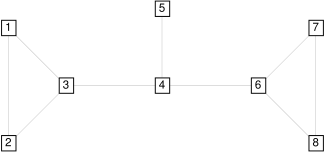
\includegraphics{graphe}
\par\end{center}

\vspace{0.3cm}


Une \emph{couverture} $C$ de ce graphe est un ensemble de sommets
qui touchent toutes les arêtes, comme par exemple $C:=\left\{ 1,3,4,7,8\right\} $:

\vspace{0.3cm}


\begin{center}
\includegraphics{graphe-couverture}
\par\end{center}

\vspace{0.3cm}

\begin{example}
On a $8$ petits villages reliés par des routes. En cas d'accident
de la route, on veut que les pompiers puissent intervenir rapidement.
Le prefet impose que lorsqu'une route relie deux villages, il y ait
une caserne de pompier dans au moins l'un des deux villages. Évidemment
le budget est serré, donc on veut construire des casernes de pompier
dans un nombre minimal de villages.

Modélisation: Chaque village est représenté par un sommet du graphe
précédent, les arêtes représentant les routes. Résoudre notre problème
revient à chercher une couverture de taille minimale du graphe.
\end{example}
Un \emph{couplage} $M$ de ce graphe est un ensemble d'arêtes qui
ne se touchent pas, comme par exemple $M:=\left\{ \left\{ 1,3\right\} ,\left\{ 4,5\right\} ,\left\{ 7,8\right\} \right\} $:

\vspace{0.3cm}


\begin{center}
\includegraphics{graphe-couplage}
\par\end{center}

\vspace{0.3cm}

\begin{example}
On veut loger un groupe de $8$ personnes dans un hotel, avec des
chambres simples et doubles. Pour minimiser les dépenses, on utiliser
le maximum de chambres doubles. D'un autre côté on ne veut pas forcer
deux personnes qui ne se connaissent pas bien à partager une chambre. 

Modélisation: chaque sommet du graphe précédent représente une personne,
et chaque arête relie deux personnes qui se connaissent bien. Résoudre
notre problème revient alors à rechercher un couplage de taille maximale
dans le graphe.\end{example}
\begin{xca}
Montrer que pour un couplage $M$ et une couverture $C$ d'un même
graphe, on a toujours $\left|M\right|\leq\left|C\right|$.
\end{xca}
%

%

%

%

%

%

\solution
\begin{proof}
Comme $C$ est une couverture, chaque arête de $M$ devra être touchée
par au moins un sommet dans $C$. De plus, $M$ étant un couplage,
chaque sommet de $C$ touche au plus une arête de $M$. Donc, on a
bien $\left|M\right|\leq\left|C\right|$.\end{proof}
\begin{problem}
Peut-on trouver $M$ et $C$ de façon à avoir égalité ?
\end{problem}
%

%

%

%

%

\solution

Dans notre exemple, non. Par contre, on va voir que pour certaines
classes de graphe, cela va être vrai: on aura un théorème de dualité
min-max. Comme par hasard, c'est une conséquence de la programmation
linéaire.

On appelle \emph{graphe biparti} un graphe dont on peut partitioner
les sommets en deux paquets $A$ et $B$ de sorte que toutes les arêtes
soient entre $A$ et $B$:

\vspace{0.3cm}


\begin{center}
\includegraphics{biparti}
\par\end{center}

\vspace{0.3cm}

\begin{xca}
On veut rechercher un couplage maximal du graphe précédent. Montrer
comment on peut résoudre ce problème en utilisant un réseau de transport.
\end{xca}
%

%

%

%

%

\solution

On peut par exemple introduire le réseau suivant. 

\vspace{0.3cm}


\begin{center}
\includegraphics{biparti-reseau}
\par\end{center}

\vspace{0.3cm}


Chaque solution entière du réseau correspond à un couplage $M$ du
graphe biparti (les arêtes sur lesquelles passent une unité). Le coût
de cette solution est $4-\left|M\right|$. Donc minimiser ce coût
revient à rechercher un couplage de taille max.

Voilà une solution arborescente optimale du réseau; on a indiqué sur
les sommets les prix relatifs, et sur les arêtes les quantités transportées:

\vspace{0.3cm}


\begin{center}
\includegraphics{biparti-reseau-optimal}
\par\end{center}

\vspace{0.3cm}


La taille maximale d'un couplage $M$ est donc $3$.

On remarque que les sommets du graphe biparti de prix $1$ à gauche
et de prix $0$ à droite (en grisé) forment une couverture optimale
de taille $3$ du graphe biparti. 
\begin{problem}
Est-ce une coïncidence?\end{problem}
\begin{xca}
Soit $T$ une solution arborescente optimale pour le réseau associé
à un graphe biparti quelconque. On définit $M$ et $C$ comme ci-dessus.
\begin{enumerate}
\item Vérifier que si $ij$ est une arête du graphe biparti, et si $i\not\in C$,
alors $j\in C$. 
\item En déduire que $C$ est une couverture du graphe biparti. 
\item Vérifier que si $i$ est dans $C$, alors $i$ appartient à une des
arêtes du couplage $M$.
\item Vérifier que si $ij$ est une des arêtes du couplage $M$, alors $i$
et $j$ ne sont pas simultanément dans $C$.
\item En déduire que $\left|M\right|=\left|C\right|$.
\end{enumerate}
\end{xca}
%

%

%

%

%Écrire la démo

\solution
\begin{thm}
(König-Egerváry) Dans tout graphe biparti, la taille d'un couplage
maximal est égale à la taille d'une couverture minimale.
\end{thm}
C'est une exemple typique où le théorème de dualité de la programmation
linéaire donne un théorème min-max reliant deux problèmes combinatoires
qui ne sont pas clairement reliés a priori.


\section{Problèmes de transports avec limites de capacités}
\begin{example*}
Modéliser un réseau routier par un réseau de transport sous forme
standard n'est pas très réaliste: sur une autoroute donnée, on ne
peut pas faire passer autant de camions que l'on veut !
\end{example*}
Dans cette section, nous allons regarder une généralisation des problèmes
de transports, dans lesquels on ajoutera des contraintes de capacités
maximales.

Nous verrons rapidement que l'algorithme du simplexe et les résultats
théoriques en découlant peuvent être étendus sans grosses difficultés.
Puis nous étudierons quelques applications.
\begin{defn*}
Problème de transport avec limites de capacités sous forme standard:

Minimiser: $cx$

Sous les contraintes: $Ax=b$ et $0\leq x\leq u$,

où $A$ est la matrice d'incidence d'un réseau.

($u$ pour \emph{upper bound}).\end{defn*}
\begin{xca*}
Peut-on mettre le problème suivant sous forme standard ?

Minimiser: $cx$

Sous les contraintes: $Ax=b$ et $l\leq x\leq u$.
\end{xca*}
%

%

%

\solution
\begin{xca*}
Donner une solution optimale pour le problème suivant:
\end{xca*}
\vspace{0.3cm}


\begin{center}
\includegraphics[width=0.75\paperwidth]{transport-cycle}.
\par\end{center}

\vspace{0.3cm}


%

%

%

%

\solution

Comme on peut le constater dans l'exercice précédent, on ne peut pas
toujours espérer trouver une solution optimale, ni même une solution
faisable arborescente: c'est-à-dire telle qu'on utilise aucune arête
en dehors d'un certain arbre $T$.

On va donc relâcher cette contrainte. Toute arête en dehors de l'arbre
$T$ devra être soit non utilisée, soit au contraire utilisée à pleine
capacité:
\begin{defn*}
Soit $T$ un arbre couvrant du réseau. 

Une solution $x$ est \emph{$T$-arborescente} si tout arc $ij\not\in T$
on a: 
\[
x_{ij}=0\textrm{ ou }x_{ij}=u_{ij}.
\]


Une solution $x$ est \emph{arborescente} s'il existe un arbre couvrant
$T$ tel que $x$ est $T$-arborescente.\end{defn*}
\begin{xca*}
Donner une solution arborescente au problème précédent.
\end{xca*}
%

%

\solution
\begin{xca*}
Étant donné un arbre $T$, a-t'on unicité de la solution arborescente
vis-à-vis de cet arbre ?
\end{xca*}
%

%

\solution
\begin{xca*}
Montrer que si les $b_{i}$ et les $u_{ij}$ sont entiers, alors toute
solution arborescente est entière.
\end{xca*}
%

%

\solution

Nous allons maintenant voir sur un exemple comment on peut adapter
l'algorithme du simplexe pour les réseaux. 

Dans le cas classique (sans limites de capacités), le principe était
de faire rentrer dans l'arbre $T$ une arête $ij$ inutilisée ($x_{ij}=0$)
rentable ($y_{i}+c_{ij}<y_{j}$) de façon à pouvoir l'utiliser.

Ici, il y a un autre cas de figure: faire rentrer une arrête $ij$
utilisée à pleine capacité ($x_{ij}=u_{ij}$) alors qu'elle n'est
pas rentable ($y_{i}+c_{ij}>y_{j}$), de façon à pouvoir diminuer
son utilisation.
\begin{example}
Cf. \cite[p.356-359]{Chvatal_LP}.\end{example}
\begin{thm*}
Soit $x$ une solution $T$-arborescente telle que pour toute arête
$ij$ en dehors de l'arbre, on ait:
\begin{itemize}
\item soit $x_{ij}=0$ et $y_{i}+c_{ij}\geq y_{j}$,
\item soit $x_{ij}=u_{ij}$ et $y_{i}+c_{ij}\leq y_{j}$.
\end{itemize}
Alors $x$ est une solution optimale.\end{thm*}
\begin{proof}
La démonstration est très similaire à celle du cas sans limites de
capacités.

On va considérer une autre solution faisable $\overline{x}$ du problème,
et comparer les coûts $cx$ et $c\overline{x}$ correspondants.

On pose $\overline{c_{ij}}:=c_{ij}-(y_{j}-y_{i})$, et $\overline{c}=[c_{ij}]$
le vecteur ligne correspondant.

$\overline{c_{ij}}$ mesure le coût relatif:
\begin{itemize}
\item $\overline{c_{ij}}=0$ si $ij$ est dans $T$
\item $\overline{c_{ij}}\geq0$ si $x_{ij}=0$ (non rentable d'utiliser
l'arc $ij$).
\item $\overline{c_{ij}}\leq0$ si $x_{ij}=u_{ij}$ (rentable d'utiliser
l'arc $ij$ à pleine capacité).
\end{itemize}
On note que dans les trois cas, $\overline{c_{ij}}\overline{x_{ij}}\geq\overline{c_{ij}}x_{ij}$.
Donc matriciellement $\overline{c}\overline{x}\geq\overline{c}x$.

Comme précédemment on peut écrire $\overline{c}$ matriciellement
sous la forme $\overline{c}=c-yA$.

De plus, $x$ et $\overline{x}$ sont solutions faisables et vérifient
donc toutes deux $Ax=b$.

On en déduit alors:
\[
c\overline{x}=\overline{c}\overline{x}+yA\overline{x}=\overline{c}\overline{x}+yb\geq\overline{c}x+yb=\overline{c}x+yAx=cx.
\]

\end{proof}

\section{Problèmes de flot maximum}


\subsection{Introduction}
\begin{defn*}
\emph{Problème de flot max:}
\begin{itemize}
\item Réseau avec source et puits
\item Pas de coûts sur les arcs
\item Contraintes de capacités sur les arcs
\item Production et consommation nulle sur chaque noeud intermédiaire
\end{itemize}
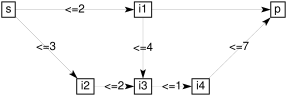
\includegraphics[width=0.75\paperwidth]{flot}

Objectif: 

Maximiser le \emph{volume} du flot, c'est-à-dire la quantité transportée
entre $s$ et $p$.\end{defn*}
\begin{example*}
Un dimanche soir, maximiser le nombre de voitures allant d'Albertville
à Lyon, en les répartissant entre les différentes routes possibles.\end{example*}
\begin{xca*}
Mettre le problème de flot dessiné ci-dessus sous forme de problème
de transport standard avec limites de capacités
\end{xca*}
%

%

%

%

\solution

Clairement, cela se généralise à tout problème de flot max.
\begin{problem*}
Que peut-on en déduire ?
\end{problem*}
%

%

%

\solution
\begin{itemize}
\item On a un algorithme de résolution (simplexe)
\item Le problème de flot est polynomial
\item On a un théorème d'intégralité:


Si les contraintes de capacités sont entières (ou infinies), alors:
\begin{itemize}
\item Soit le problème est non borné: \includegraphics{flot-nonborne}
\item Soit le problème a une solution entière
\end{itemize}
\item On doit bien avoir une dualité !
\end{itemize}

\subsection{Dualité: le théorème flot max / coupe min}
\begin{defn*}
Une \emph{coupe} $C$ dans un réseau est un ensemble de sommets du
réseau contenant la source.

La capacité de la coupe $C$ est la somme des capacités des arrêtes
sortantes de $C$.\end{defn*}
\begin{example*}
Dans notre réseau, la coupe $C=\left\{ s\right\} $ est de capacité
$5$.
\end{example*}
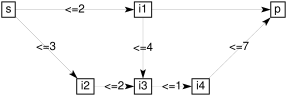
\includegraphics[width=0.75\paperwidth]{flot}
\begin{xca*}
Quelle est la capacité de la coupe $C=\left\{ s,i_{2},i_{3}\right\} $?

Que peut-on en déduire sur la valeur d'un flot ?
\end{xca*}
%

%

%

%

%

\solution
\begin{prop*}
Pour toute coupe $C$ et tout flot $F$ dans un réseau, la capacité
$\left|C\right|$ de la coupe est supérieure au volume $\left|F\right|$
du flot: $\left|C\right|\geq\left|F\right|$.\end{prop*}
\begin{problem*}
Que peut on espérer avoir ?
\end{problem*}
%

%

\solution

Une dualité et un théorème min-max, bien-sûr!
\begin{thm*}
(Coupe min-Flot max) Dans un réseau, le volume maximal d'un flot est
égal à la capacité minimale d'une coupe.\end{thm*}
\begin{xca*}
Vérifiez-le dans notre exemple.\end{xca*}
\begin{proof}
On considère une solution $F$ optimale du problème de flot obtenue
avec le simplexe pour les réseaux avec limites de capacité.

\includegraphics[width=0.75\paperwidth]{flot-reseau}

On calcule les valeurs $y_{i}$ en chaque sommets.

Les coûts sont de $0$ partout sauf sur l'arc $ps$, où le coût est
de $-1$.

Donc la valeur de $y_{i}$ est:
\begin{itemize}
\item $0$ si $i$ est relié à $s$ dans $T$,
\item $1$ si $i$ est relié à $t$ dans $T$.
\end{itemize}
On prend comme coupe $C$ l'ensemble des sommets $i$ avec $y_{i}=0$.

Chaque arc $ij$ sortant de $C$ est «rentable» puisque $y_{i}+c_{ij}=0<1=y_{j}$.

Or, $ij$ n'est pas dans l'arbre, et le flot est optimal.

Donc $ij$ doit être utilisé à pleine capacité: $x_{ij}=u_{ij}$.

De même, tout arc $ij$ entrant est non rentable, et n'est donc pas
utilisé: $x_{ij}=0$.

Conclusion: Le volume du flot $F$ est égal à la capacité de la coupe
$C$:

\[
\left|F\right|=\sum_{ij\textrm{ sortant}}x_{ij}-\sum_{ij\textrm{ entrant}}x_{ij}=\sum_{ij\textrm{ sortant}}u_{ij}=\left|C\right|.
\]
\end{proof}
\begin{rem*}
Il y a quelques boulons à serrer.
\begin{enumerate}
\item Le simplexe pourrait terminer en indiquant que le problème est non
borné: \emph{i.e.} il existe des flots de volume aussi grand que l'on
veut:


\vspace{0.3cm}



\begin{center}
\includegraphics[width=0.5\paperwidth]{flot-reseau-nonborne}
\par\end{center}


\vspace{0.3cm}



Dans ce cas, il ne peut pas y avoir de coupe de capacité finie. 


Donc le théorème reste valide.

\item Le simplexe pourrait indiquer que le problème est non faisable.


En fait, non, puisque $x_{ij}=0,\textrm{ }\forall x_{ij}$ est solution.

\item Si le flot max est de volume $0$, il se pourrait que l'arbre ne contienne
pas l'arc $ps$. Du coup, l'ensemble des sommets $i$ tels que $y_{i}=0$
ne serait pas forcément une coupe.


Un tel cas correspond en fait à une solution dégénérée qui est arborescente
vis-à-vis de plusieurs arbres. 


En fait, en faisant un pivot convenable, on peut toujours remettre
$ps$ dans l'arbre.

\end{enumerate}
\end{rem*}

\subsection{Applications}

On a vu que les problèmes de flots était un cas particulier des problèmes
de transport avec limites de capacités.

Quel est donc l'intérêt de considérer les problèmes de flots ?

On a un algorithme (méthode du chemin augmentant) plus rapide que
le simplexe.


\subsubsection{Trouver une solution faisable dans un problème de transport avec
limites de capacités}
\begin{example*}
On prend le problème de transport suivant, et on se demande s'il est
faisable.

\vspace{0.3cm}



\begin{center}
\includegraphics[width=0.75\paperwidth]{flot-transportfaisable}
\par\end{center}


\vspace{0.3cm}


On peut le transformer en problème de flot, en oubliant les coûts,
et en rajoutant une source, reliée convenablement aux producteurs,
et un puits, relié convenablement aux consommateurs:

\vspace{0.3cm}



\begin{center}
\includegraphics[width=0.75\paperwidth]{flot-transportfaisable2}
\par\end{center}


\vspace{0.3cm}


S'il existe un flot de volume $8$, les arcs reliant $s$ aux producteurs
seront utilisés à pleine capacité, et de même pour les arcs reliant
les consommateurs à $t$. Cela simule exactement les productions et
consommations escomptées, donc le problème de réseau d'origine est
faisable.

La réciproque est aussi clairement vraie: si le problème est faisable,
alors il existe un flot de volume $8$.

Dans notre cas, on en déduit que le problème n'est pas faisable. En
effet, on peut trouver une coupe de capacité $7$.
\end{example*}
De manière générale, on peut toujours transformer un problème de transport
avec limite de capacité en un problème de flot, de façon à déterminer
s'il est faisable.

Cela donne un algorithme plus rapide que le simplexe pour la phase
I de la résolution.


\subsubsection{Couplages dans les graphes bipartis}
\begin{xca*}
Mettre sous forme de problème de flot le problème de rechercher un
couplage max dans le graphe biparti suivant.
\end{xca*}
\vspace{0.3cm}



\subsubsection{Problème des mines à ciel ouvert}
\begin{problem*}
Des études géologiques ont permis de déterminer précisément la nature
du sous-sol, et l'emplacement des gisements orifères à l'endroit ou
l'on a décidé de creuser une mine à ciel ouvert. Certains gisements
sont profonds, et il n'est pas clair qu'il soit rentable d'excaver
tout le sol au-dessus pour y accéder.

Modèle: le sous-sol a été délimité en un certain nombre de blocs.
Pour chaque bloc $i$, on connaît le coût $C_{i}$ d'excavation, et
le profit $P_{i}$ que l'on peut escompter de son traitement.

Au final, on associe à chaque bloc $i$ la quantité $w_{i}=C_{i}-P_{i}$.
Si l'on ne considère pas les autres blocs, il est rentable de creuser
$i$ si et seulement si $w_{i}<0$.

On veut déterminer quels blocs on doit creuser pour maximiser le profit
total $-\sum_{i}w_{i}$ (ou autrement dit minimiser $\sum_{i}w_{i}$).

Maintenant, il y a des contraintes supplémentaires: si un bloc $i$
est sous un bloc $j$, on ne peux pas creuser $i$ sans creuser $j$!

On introduit un ordre partiel, de sorte que $i<j$ si pour creuser
$i$ on doit creuser $j$.

Comme on le verra, la forme des blocs, et le type d'ordre partiel
n'est pas relevant.\end{problem*}
\begin{example*}
On considère le sous-sol suivant:
\end{example*}
Comment modéliser notre problème sous forme de problème de flot max
?

La modélisation des contraintes de précédences est un peu astucieuse!

On introduit le réseau suivant:

C'est la remarque suivante qui va faire marcher la machine:
\begin{rem*}
Soit $C$ une coupe. 

S'il existe deux blocs $i<j$, avec $i\in C$ et $j\in C$, alors
$C$ est de capacité infinie.

La réciproque est vraie.
\end{rem*}
Les coupes de capacité finie sont en correspondance avec les coupes
respectant les contraintes.

Maintenant, on peut vérifier que la capacité d'une coupe finie vaut
exactement

\[
\sum_{i\in C,\textrm{ }i\textrm{ bloc non rentable}}w_{i}-\sum_{i\not\in C,\textrm{ }i\textrm{ bloc rentable}}w_{i}.
\]


Quitte à rajouter le terme constant $\sum_{i,\textrm{ }i\textrm{ bloc}}w_{i}$,
on est en train de calculer le profit lorsque l'on enlève les blocs
$i$ avec $i\in C$.

Résumé: Soit $I$ un ensemble de blocs, et $C$ la coupe $\left\{ s\right\} \cup I$.
\begin{itemize}
\item Si $I$ ne satisfait pas les contraintes, la capacité de $C$ est
infinie.
\item Si $I$ satisfait les contraintes, la capacité de $C$ est l'opposé
du profit.
\end{itemize}
Maximiser le profit revient à trouver une coupe min.
\begin{rem*}
En termes pédants: on peut résoudre par un algorithme de flot le problème
de trouver une section finale de poids minimal dans un ordre partiel.
\end{rem*}

\subsubsection{Dualités chaînes/antichaînes dans les ordres partiels; théorème de
Dilworth}
\begin{problem}
\cite[p. 338]{Chvatal_LP} Problème des visites guidées. Une compagnie
propose $7$ visites guidées dans la journée, notées $a,b,c,d,e,f,g$,
dont les horaires et durées sont fixées. Si une visite (par ex. $a$)
termine suffisament avant une autre (par exemple $c$), le guide de
la première visite peut enchaîner sur la deuxième; on notera alors
$a\rightarrow c$. En l'occurence, voici tous les enchaînements possibles:

$a\rightarrow c,\textrm{ }a\rightarrow d,\textrm{ }a\rightarrow f,\textrm{ }a\rightarrow g,\textrm{ }b\rightarrow c,\textrm{ }b\rightarrow g,\textrm{ }d\rightarrow g,\textrm{ }e\rightarrow f,\textrm{ }e\rightarrow g$.
\begin{itemize}
\item Combien faut-il de guides au minimum dans cet exemple ?
\item Comment trouver le nombre minimum de guides nécessaires dans le cas
général ?
\end{itemize}
\end{problem}
%

%

%

%

%

%

\solution
\begin{defn*}
Soit $P=(E,<)$ un ordre partiel. 

Une \emph{chaîne} $C$ de $P$ est un ensemble de sommets de $P$
deux à-deux comparables:
\[
x\in C\textrm{ et }y\in C\textrm{ }\Rightarrow\textrm{ }x<y\textrm{ ou }y<x.
\]


Une \emph{antichaîne} $A$ de $P$ est un ensemble de sommets deux-à-deux
incomparables.

Une \emph{couverture en chaînes} de $P$ est un ensemble $C_{1},\ldots,C_{k}$
de chaînes, de sorte que tout sommet de $P$ est dans une unique chaîne
$C_{i}$.

Une \emph{couverture en antichaînes} de $P$ est un ensemble $A_{1},\ldots,A_{k}$
d'antichaînes, de sorte que tout sommet de $P$ est dans une unique
antichaîne $A_{i}$.\end{defn*}
\begin{xca}
Trouver dans l'ordre partiel $P$ précédent:
\begin{enumerate}
\item Une chaîne de taille maximale
\item Une antichaîne de taille maximale
\item Une couverture en chaînes de $P$ de taille minimale
\item Une couverture en antichaînes de $P$ de taille minimale
\end{enumerate}
Que remarquez vous ?
\end{xca}
%

%

%

\solution

Y-aurait-il un théorème min-max reliant la taille de la plus grande
chaîne et la taille de la plus petite couverture en antichaînes ?
Et un autre reliant la taille de la plus grande antichaîne et celle
de la plus petite couverture en chaînes ?
\begin{xca}
Soit $P$ un ordre partiel quelconque.
\begin{enumerate}
\item Soit $C$ une chaîne de $P$ et $A_{1},\ldots,A_{k}$ une couverture
de $P$ en antichaînes.


Montrer que $\left|C\right|\leq k$.

\item Soit $A$ une antichaîne de $P$ et $C_{1},\ldots,C_{k}$ une couverture
de $P$ en chaînes.


Montrer que $\left|A\right|\leq k$.

\end{enumerate}
\end{xca}
\begin{prop}
Soit $P$ un ordre partiel. La taille de la plus grande chaîne de
$P$ est égale à la taille de la plus petite couverture en antichaînes
de $P$.\end{prop}
\begin{xca}
Prouvez-le!
\end{xca}
%

%

%

%

%

\solution

Le théorème dans l'autre sens est plus difficile et bien plus profond.
Il n'y a pas de construction élémentaire de l'antichaîne et de la
couverture en chaîne idoine. On va en fait se ramener à la programation
linéaire (surprise).
\begin{thm}
(Dilworth) Soit $P$ un ordre partiel. La taille de la plus grande
antichaîne de $P$ est égale à la taille de la plus petite couverture
en chaînes de $P$.\end{thm}
\begin{proof}
On note $n$ le nombre de sommets de $P$. 

Choisir une couverture en chaîne de $P$ est équivalent à sélectionner
un certain nombre d'arcs dans $P$, de sorte que chaque sommet ait
au plus un arc sortant de sélectionné, et un arc rentrant de sélectionné. 

Remarque: s'il y a $k$ chaînes, il y a $n-k$ arcs sélectionnés.

Cela ressemble à un problème de couplage maximal dans un graphe biparti.

On construit un graphe biparti $B$ dans lequel chaque sommet $x$
de $P$ est dupliqué en $(x,1)$ et $(x,2)$. 

Chaque fois que $x<y$ dans $P$, on relie $(x,1)$ et $(y,2)$.

Qu'est-ce qu'un couplage dans $B$?

Un ensemble d'arcs de $P$ vérifiant exactement les conditions voulues.

Une couverture de $P$ en $k$ chaînes correspond à un couplage de
$B$ de taille $n-k$.

Prenons une couverture de $P$ de taille $k$ minimale.

Cela donne un couplage de taille max $n-k$ de $B$.

Le théorème min-max pour les graphes bipartis indique qu'il y a une
couverture de $B$ de même taille: $n-k$ sommets de $B$ qui touchent
tous les arcs.

Dans $P$ cela correspond à au plus $n-k$ sommets qui touchent tous
les arcs.

Soit $A$ l'ensemble des sommets restants qui est de taille au moins
$k$.

Il ne peut pas y avoir d'arcs entre deux sommets de $A$. 

Conclusion: $A$ est une antichaîne de taille au moins $k$.\end{proof}
\begin{xca}
Suivez le déroulement de la preuve sur l'ordre partiel précédent
\end{xca}

\subsection{La méthode du chemin augmentant}

Rechercher un couplage max dans un graphe biparti est un problème
très classique.

Il existe en fait des techniques plus rapides que les algorithmes
de réseaux de transport.

L'une d'entre elles est la méthode du chemin augmentant.


\subsubsection{Cas général des graphes simples}
\begin{example}
Couplage de taille maximale dans le chemin $P_{6}$.

On peut construire un couplage de taille maximal progressivement à
partir d'un couplage vide en rajoutant des arêtes une à une. Mais
si on n'est pas parti correctement, on risque d'être bloqué avec un
couplage qui est maximal, alors qu'il n'est pas de taille maximale.
Il faut appliquer une transformation au couplage pour pouvoir l'agrandir.\end{example}
\begin{defn}
Soit $M$ un couplage dans un graphe $G$. 

Un sommet \emph{$M$-saturé} (ou saturé) est un sommet touchant une
arête du couplage.

Un chemin \emph{$M$-alterné} de $G$ est un chemin de $G$ qui utilise
alternativement des arêtes dans $M$ et hors de $M$.

Un chemin \emph{$M$-augmentant} est un chemin $M$-alterné commençant
et finissant par des sommets non $M$-saturés.\end{defn}
\begin{example}
Regardons ce que cela donne avec le couplage suivant:

\vspace{0.3cm}



\begin{center}
\includegraphics{couplage2}
\par\end{center}


\vspace{0.3cm}


\end{example}
\begin{rem*}
Si $M$ est un couplage, et $C$ est un chemin $M$-augmentant, alors
on peut construire un couplage $M'$ strictement plus grand en utilisant
$C$.

Cas particulier: lorsque le chemin $M$-augmentant consiste d'une
seule arête reliant deux sommets non saturés, on est ramené au rajout
d'une arête au couplage $M'$.\end{rem*}
\begin{xca*}
Soit $G$ le graphe

\vspace{0.3cm}



\begin{center}
\includegraphics{couplage}
\par\end{center}


\vspace{0.3cm}


Le couplage $M$ dessiné est maximal, mais pas de taille maximale.
Trouvez un chemin $M$-augmentant et construisez le couplage $M'$
correspondant.
\end{xca*}
Est-ce que cette opération de chemin augmentant est suffisante ?
\begin{thm*}
(Berge 1957) Un couplage $M$ est de taille maximale si et seulement
s'il n'y a pas de chemin $M$-augmentant.\end{thm*}
\begin{proof}
Soit $M$ un couplage, comme dans l'exemple suivant:

\vspace{0.3cm}



\begin{center}
\includegraphics{couplage-berge}
\par\end{center}


\vspace{0.3cm}


On suppose qu'il existe un couplage $M'$ de taille strictement plus
grande.

\vspace{0.3cm}



\begin{center}
\includegraphics{couplage-berge2}
\par\end{center}


\vspace{0.3cm}


On va construire un chemin $M$-augmentant.

On considère le graphe $H$ obtenu par réunion de $M$ et $M'$.

Les sommets de $H$ sont de degré au plus $2$.

Ses composantes connexes sont donc des doubles arêtes ou des cycles
et chemins dont les arêtes alternent entre $M$ et $M'$. Dans un
cycle ou une double arête il y a autant d'arêtes de $M$ que de $M'$.
Il y aura donc forcément un chemin qui contiendra une arête de plus
de $M'$ que de $M$. Ce chemin est un chemin $M$-augmentant.
\end{proof}
On déduit de ce théorème un algorithme (ou plutôt une méthode):
\begin{algorithm}
Recherche d'un couplage maximal dans un graphe:\end{algorithm}
\begin{enumerate}
\item Partir d'un couplage $M$ quelconque (par exemple le couplage vide);
\item Chercher un chemin $M$-augmentant;
\item S'il n'y en a pas, renvoyer $M$ qui est maximal; sinon réitérer avec
$M:=M'$.\end{enumerate}
\begin{xca*}
Appliquez cette méthode pour trouver un couplage maximal du graphe
\end{xca*}
\vspace{0.3cm}


\begin{center}

\includegraphics{biparti2}
\par\end{center}

\vspace{0.3cm}


Pour un graphe quelconque, l'étape 2 peut être difficile!

Par contre, pour un graphe biparti, il y a un algorithme.


\subsubsection{Recherche d'un chemin augmentant pour un couplage d'un graphe biparti}
\begin{example*}
On va rechercher un couplage maximal dans le graphe biparti précédent,
en montrant comment on peut trouver de manière systématique un chemin
$M$-augmentant.\end{example*}
\begin{algorithm}
Soit $M$ un couplage d'un graphe biparti $B$ entre les parties $X$
et $Y$.

Cet algorithme renvoie soit un chemin $M$-augmentant, soit une couverture
du graphe de taille $\left|M\right|$, ce qui indiquera que le couplage
$M$ est de taille maximale.

Soit $U$ l'ensemble des sommets de $X$ non touchés par $M$, et
$V$ l'ensemble des sommets de $Y$ non touchés par $M$.

On va rechercher par un parcours en largeur les chemins $M$-alternés
allant de $U$ à $V$.

$S$ (resp. $T$) va représenter l'ensemble des sommets $x$ de $X$
(resp. $Y$) pour lesquels on aura déjà trouvé un chemin $M$-alterné
allant de $U$ à $x$.
\begin{description}
\item [{Initialisation:}] $S:=U$, $T:=\emptyset$;
\item [{Itération:}]~

\begin{description}
\item [{Cas~1:}] Il y a une arête reliant un sommet de $S$ à un sommet
de $V$. Cela donne un chemin $M$-augmentant que l'on renvoie
\item [{Cas~2:}] Il y a une arête reliant un sommet $x$ de $S$ à un
sommet $y$ de $Y-V$ avec $xy\notin\not M$. Ce sommet est relié
par une arête du couplage à un sommet $w$ de $X$. Comme $y$ et
$w$ sont reliés à $U$ par un chemin $M$-alterné, on rajoute $y$
à $T$ et $w$ à $S$.
\item [{Cas~3:}] $T\cup(X-S)$ est une couverture de taille $\left|M\right|$
du graphe (vérifiez le!) que l'on renvoie.
\end{description}
\end{description}
\end{algorithm}
\begin{xca}
Appliquer l'algorithme sur un graphe biparti de votre choix

Démontrer que $T\cup(X-S)$ est bien une couverture de taille $\left|M\right|$
du graphe.
\end{xca}
Donner la preuve


\subsection{Algorithme de Ford-Fulkerson}

La méthode du chemin augmentant se généralise à la recherche de couplage
max dans un graphe biparti valué, et en fait aussi aux problèmes de
flots max. On ne va regarder son fonctionnement que sur un exemple,
et on renvoie à \cite[p.~369]{Chvatal_LP} pour les détails.
\begin{example*}
On veut transporter le plus grand nombre possible de voyageurs de
San-Francisco à New-York, sachant qu'il ne reste que quelques places
dans les avions entre les villes suivantes:

\vspace{0.3cm}



\begin{center}
\includegraphics[width=0.75\paperwidth]{flot-voyageurs}
\par\end{center}


\vspace{0.3cm}


\end{example*}
\begin{defn*}
Soit $R$ un réseau, et $F$ un flot donné dans ce réseau.

Un chemin allant de la source $s$ au puits $p$ est \emph{$F$-augmentant}
si pour chaque arête $ij$ du chemin on a:
\begin{itemize}
\item $x_{ij}<u_{ij}$ si l'arc $ij$ est dans le même sens que dans le
réseau
\item $x_{ij}>0$ si l'arc $ij$ est dans le sens inverse du réseau.
\end{itemize}
\end{defn*}
À partir d'un chemin $F$-augmentant, on peut construire un nouveau
flot $F'$ qui sera de volume strictement plus gros.

Le principe de l'algorithme de Ford-Fulkerson est de partir d'un flot
$F$ quelconque, et de l'améliorer itérativement en recherchant des
chemins $F$-augmentant.

À chaque étape, la recherche d'un chemin $F$-augmentant se fait par
un parcours en profondeur, de manière similaire à la recherche d'un
chemin $M$-augmentant dans un graphe biparti. Si cette recherche
échoue, elle dévoile une coupe de capacité égale au flot, ce qui donne
un certificat d'optimalité du flot.
\begin{rem*}
On peut toujours initialiser l'algorithme avec un flot nul.

Si toutes les capacités sont entières et finies, chaque itération
augmente le flot d'au moins $1$. Cet algorithme ne peut donc pas
cycler, et il termine en un nombre fini d'étapes.

Avec une mauvaise stratégie, et des capacités infinies ou non-entières,
l'algorithme peut ne pas terminer.

\vspace{0.3cm}



\begin{center}
\includegraphics{flot-mauvais}
\par\end{center}


\vspace{0.3cm}


Avec une stratégie convenable, cet algorithme est en fait polynomial,
en $O\left(n^{3}\right)$, même si les capacités sont infinies ou
non entières.

Pour les réseaux avec peu d'arcs, il y a des algorithmes plus compliqués
qui permettent d'obtenir d'encore meilleurs bornes. Cf. \cite[p.~369]{Chvatal_LP}
pour les détails.
\end{rem*}

\section{Méthodes alternatives au simplexe}

Pour conclure ce chapitre sur la programmation linéaire, nous présentons
rapidement quelques méthodes alternatives qui ont été développées
pour résoudre les problèmes de programmation linéaire généraux. Nous
nous contentons d'évoquer leur principe, leurs avantages et inconvénients,
et donnons des références pour ceux qui voudraient en savoir plus.


\subsection{Méthode de l'ellipsoïde}
\begin{description}
\item [{Principe}] On commence par utiliser la dualité pour se ramener
à la recherche d'une solution faisable d'un système d'inéquations
linéaires. On peut en fait se ramener par une perturbation convenable
à la recherche d'une solution faisable d'un système d'inéquations
linéaires strictes!


Si un tel système est faisable, le volume de l'ensemble des solutions
peut alors être minoré par une quantité $V$ qui dépends de la dimension
de l'espace, et de la taille des coefficients dans le système linéaire.


On part d'un ellipsoïde $E$ suffisamment gros pour contenir toutes
les solutions faisables.


Si le centre de $E$ est une solution faisable, on a terminé.


Sinon, on peut couper l'ellipsoïde en deux, et inclure ce demi-ellispoïde
dans un ellipsoïde $E'$ qui contient encore toutes les solutions
faisables. On réitère avec $E:=E'$.


À chaque itération, on a $V(E')<\alpha V(E)$, où $\alpha<1$ est
une constante qui ne dépends que de la dimension; donc le volume de
$E$ décroît exponentiellement. Au bout d'un petit nombre d'itérations,
si l'on a pas obtenu de solution faisable, on a $V(E)<V$, ce qui
prouve que la système n'a pas de solution faisable.

\item [{Avantages}]~

\begin{itemize}
\item Algorithme polynomial
\end{itemize}
\item [{Inconvénients}]~

\begin{itemize}
\item Plus lent \emph{en pratique} que l'algorithme du simplexe
\item Ne donne pas certains résultats théoriques (dualité, géométrie des
polyèdres)
\end{itemize}
\item [{Référence}] \cite[p.~443]{Chvatal_LP}
\end{description}

\subsection{Méthode des points intérieurs}
\begin{description}
\item [{Principe}] Cette méthode est l'antithèse exacte du simplexe. 


Le principe du simplexe est de ne considérer que des solutions basiques
qui sont à la frontière du polyèdre, et d'utiliser de l'algèbre linéaire
pour itérer parmi ces solutions.


Ici au contraire, la méthode ne considère que des solutions strictement
à l'intérieur du polyèdre. L'idée est d'approximer les inégalités
du système linéaire, qui forment fondamentalement des discontinuités,
en barrières de potentiel, qui sont elles continues. Du coup, on peut
utiliser les techniques d'optimisation non-linéaire continue, comme
les méthodes de gradients.

\item [{Avantages}]~

\begin{itemize}
\item Rivalise avec le simplexe \emph{en pratique}, suivant le type de problème
rencontrés
\end{itemize}
\item [{Inconvénients}]~

\begin{itemize}
\item Ne donne pas de résultats théoriques (dualité, géométrie des polyèdres)
\end{itemize}
\item [{Références}] \cite{Vanderbie_LPFE}\end{description}
\begin{thebibliography}{1}
\bibitem{Chvatal_LP}V.~Chvatal. Linear Programming.

\bibitem{Vanderbie_LPFE}R.~Vanderbie. Linear Programming; Foundations
and Extensions. \url{http://www.princeton.edu/~rvdb/LPbook/index.html}

\bibitem{LP_FAQ}Linear Programming FAQ \url{http://rutcor.rutgers.edu/~mnk/lp-faq.html}

\bibitem{Wikipedia}\url{http://en.wikipedia.org/wiki/Linear_programming}\end{thebibliography}

\end{document}
